\documentclass{VUMIFInfBakalaurinis}
\usepackage{algorithmicx}
\usepackage{algorithm}
\usepackage{algpseudocode}
\usepackage{amsfonts}
\usepackage{amsmath}
\usepackage{bm}
\usepackage{caption}
\usepackage{color}
\usepackage{float}
\usepackage{graphicx}
\usepackage{listings}
\usepackage{subfig}
\usepackage{url}
\usepackage{wrapfig}

\usepackage{longtable}
\usepackage{rotating}

\usepackage{amsbsy}

\usepackage{enumitem}

\usepackage{hyperref} %[pdfpagelabels,bookmarks,hyperindex,hyperfigures]
\usepackage{xcolor}

%\definecolor{mygray}{rgb}{0.5,0.5,0.5}
%\lstset{ %
%  numbers=left,                    	% where to put the line-numbers;
%  numbersep=5pt,                   	% how far the line-numbers are from the code
%  numberstyle=\tiny\color{mygray}, 	% the style that is used for the line-numbers
%  breaklines=true,                 	% sets automatic line breaking
%  frame=single,	                   	% adds a frame around the code
%  morekeywords={of,in},				% if you want to add more keywords to the set
%  tabsize=2	                   		% sets default tabsize to 2 spaces
%}

%if errors .aux, .toc

\hypersetup{
    bookmarks=true,         % show bookmarks bar?
    %unicode=false,          % non-Latin characters in Acrobat’s bookmarks
    %pdftoolbar=true,        % show Acrobat’s toolbar?
    %pdfmenubar=true,        % show Acrobat’s menu?
    %pdffitwindow=false,     % window fit to page when opened
    %pdfstartview={FitH},    % fits the width of the page to the window
    pdftitle={Dalykinės srities modelio transformavimas į UML užduočių diagramas},    % title
    pdfauthor={Aleksandras Sivkovas},     % author
    hidelinks
}

\newcommand{\bref}[1]{\textbf{\ref{#1}}}
\newcommand{\bhyperref}[2]{\hyperref[#1]{\textbf{#2}}}
\newcommand{\DVCM}{\bhyperref{section:dvcm}{DVGM}}
\newcommand{\BPMN}{\bhyperref{section:bpmn}{BPMN}}
\newcommand{\OMG}{\bhyperref{def:omg}{OMG}}
\newcommand{\UML}{\bhyperref{def:uml}{UML}}
\newcommand{\SysML}{\bhyperref{def:sysml}{SysML}}
\newcommand{\JSON}{\bhyperref{def:json}{JSON}}
\newcommand{\inCode}[1]{\fcolorbox{black}{white}{\lstinline{#1}}}
\newcommand{\uiWord}[1]{„#1“}


%\definecolor{dkgreen}{rgb}{0,0.6,0}
%\definecolor{gray}{rgb}{0.5,0.5,0.5}
%\definecolor{mauve}{rgb}{0.58,0,0.82}
%\definecolor{light-gray}{gray}{0.25}
%keywordstyle=\bfseries\color{blue},
%  commentstyle=\itshape\color{dkgreen},
%  stringstyle=\color{mauve},

\lstdefinestyle{pseudocode}{
  language=Java,
  aboveskip=3mm,
  belowskip=3mm,
  showstringspaces=false,
  columns=flexible,
  basicstyle={\normalsize\ttfamily},
  numberstyle={\tiny},
  numbers=left,
  keywordstyle=\pmb,
  commentstyle=\itshape,
  stringstyle=\itshape,
  breaklines=true,
  breakatwhitespace=true,
  tabsize=2,
  morekeywords={of,in,function},
  escapeinside={(*}{*)},          % if you want to add LaTeX within your code
  frame=single	                   	% adds a frame around the code
}

\lstdefinestyle{javascript}{
  language=Java,
  aboveskip=3mm,
  belowskip=3mm,
  showstringspaces=false,
  columns=flexible,
  basicstyle={\normalsize\ttfamily},
  numberstyle={\tiny},
  numbers=left,
  keywordstyle=\pmb,
  commentstyle=\itshape,
  stringstyle=\itshape,
  breaklines=true,
  breakatwhitespace=true,
  tabsize=2,
  morekeywords={of,in,function},
  escapeinside={(*}{*)},          % if you want to add LaTeX within your code
  frame=single	                   	% adds a frame around the code
}

\lstset{
  morekeywords={of,in,function}
}


%%% Table of contents to list down to subsections and no further
\setcounter{tocdepth}{4}

%%% Number down to subsubsections only
\setcounter{secnumdepth}{4}

% Titulinio aprašas
\university{Vilniaus universitetas}
\faculty{Matematikos ir informatikos fakultetas}
\department{Programų sistemų katedra}
\papertype{Baigiamasis bakalauro darbas}
\title{Dalykinės srities modelio transformavimas į UML užduočių diagramas}
\titleineng{Deriving use cases from business process}
\status{4 kurso 1 grupės studentas}
\author{Aleksandras Sivkovas}
% \secondauthor{Vardonis Pavardonis}   % Pridėti antrą autorių
\supervisor{Prof. dr. Saulius Gudas}
\reviewer{prof. dr. Romas Baronas}
\date{Vilnius \\ \the\year}

% Nustatymai
% \setmainfont{Palemonas}   % Pakeisti teksto šriftą į Palemonas (turi būti įdiegtas sistemoje)
\bibliography{bibliografija}

\begin{document}

\newcounter{counter:table:reset}
\newcounter{counter:table}[counter:table:reset]
\newcommand\rownumber{\stepcounter{counter:table}\arabic{counter:table}}

\maketitle

\sectionnonumnocontent{Santrauka}

Darbe rašoma apie sistemos funkcinių reikalavimų gavimą užduočių diagramos pavidalu iš dalykinės srities modelio. Parodomas reikalavimų inžinerijos bei įrankio šiam procesui atlikti aktualumas. Įrankis padėtų sumažinti klaidų kiekį, paspartintų procesą, jis leistų dalintis reikalavimais ir sekti jų pasikeitimus. Darbe nagrinėjami BPMN, UML ir SysML standartai bei pasiūlomi jų išplėtimai apibrėžiantys modelius reikalavimų inžinerijos automatizavimui. Taip pat pateikiamas algoritmas užduočių diagramos gavimui iš pasiūlyto BPMN išplėtimo ir aprašoma sukurta programa demonstruojanti jo veikimą.

% Nurodomi iki 5 svarbiausių temos raktinių žodžių (terminų).
% Vienas terminas gali susidėti iš kelių žodžių.
\raktiniaizodziai{BPMN, Užduočių diagrama, UML, SySML, DVGM}

\sectionnonumnocontent{Summary}
The paper describes how to obtain the functional requirements of the system in the form of the use cases from business process. The relevance of requirement engineering and a tool for it is shown. The usage of tool would to reduce the amount of errors, speed up the process, allow sharing of requirements and tracking their changes. The paper analyses the standards of BPMN, UML and SysML, and proposes their extensions that could be used for automation of requirement engineering process. Also the algorythm for deriving use cases from extended BPMN and description of tool to demonstrate algorythm is provided.
\keywords{BPMN, Use cases, UML, SySML, DVCM}

\tableofcontents

%xelatex bakalaurinis.tex|biber bakalaurinis|xelatex bakalaurinis.tex|evince %.pdf
%xelatex %.tex|biber %|xelatex %.tex|evince %.pdf

\sectionnonum{Įvadas}

Reikalavimų inžinerija yra svarbi programų kūrimo dalis. Tai yra akivaizdus dalykas naudojant tradicines programų kūrimo metodologijas, bet ir pastarąjį dešimtmetį pripažinimo sulaukusiose judriose metodologijose, svarbu žinoti kokia sistema yra kuriama. Straipsnis \cite{reInAgile} kalba apie reikalavimų inžinerijos ypatumus ir trūkumus judriose metodologijose. \cite{jacobson2011usecase} parodoma kaip užduočių diagramos galėtų būti naudojamos judriose metodologijose. Taip pat, dėl didesnių galimybių susirasti įgudusių programų sistemų inžinierių, organizacijos vis labiau ima taikyti „globalų programų sistemų kūrimo metodą“.  \cite{reInGlobalPrograming} kalba apie reikalavimų inžineriją paskirstytose komandose (distributed teams). Viena iš straipsnio analizės išvadų yra „There Need To Be A Shared Understanding Between Teams About How Requirements Changes Would Be Dealt With“. Autoriai siūlo naudoti įrankį reikalavimų analizei ir sistemiškai tvarkingam reikalavimų specifikavimui.

Reikalavimų inžinerija yra sudėtinga programų kūrimo dalis. Proceso sudėtingumas dažnai tampa klaidų priežastimi. Čia atsiradusios klaidos sunkiai aptinkamos ir sukelia brangiai kainuojančias pasekmes, nes sekančiuose etapuose bus kuriama neteisingai apibrėžta programa. Norint išvengti klaidų galima kai kurias proceso veiklas automatizuoti. Nors yra daug modeliavimo įrankių, juose trūksta automatinio vieno modelio generavimo iš kito.

Projektuojant sistemą gali atsitikti toks atvejis (\ref{img:bad_model_use_cases} pav.). Čia pavaizduota, kad analitikas aptiko kokias funkcijas reikia įgyvendinti. Analizuodamas \ref{img:bad_model} pav. pavaizduotą veiklą jis aptiko vartojimo atvejus pažymėtus 1, 2, 3, 5. Taigi nuspręsta kurti sistemą pavaizduotą  \ref{img:bad_model_use_cases} pav.

\begin{figure}[H]
	\centering
	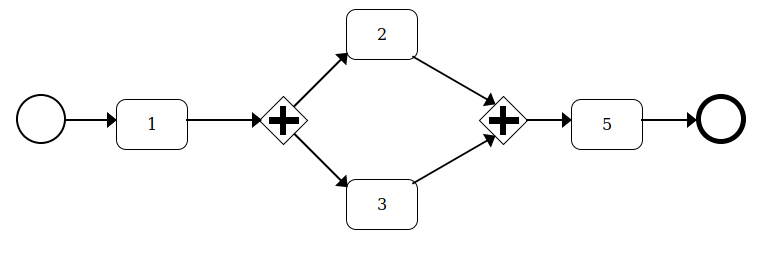
\includegraphics[width=\textwidth]{img/bad_modeling/bad_model}
	\caption{Veiklos modelio pavyzdys}
	\label{img:bad_model}
\end{figure}
\begin{figure}[H]
	\centering
	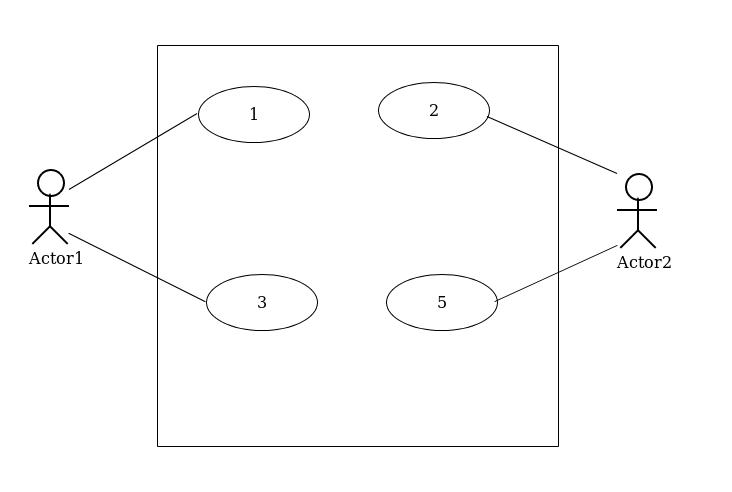
\includegraphics[width=15cm]{img/bad_modeling/bad_model_use_cases}
	\caption{Vartojimo atvejų diagramos sukurtos pagal \ref{img:bad_model} pav. veiklą pavyzdys}
	\label{img:bad_model_use_cases}
\end{figure}

Bet vėliau paaiškėjo, kad norint įgyvendinti veiklą pažmėtą 5 kartais reikia duomenų iš 4 veiklos pažymėtos punktyrine linija (\ref{img:corrected_model} pav.). Taigi vartojimo atvejų diagramoje trūko 4 vartojimo atvejo (\ref{img:corrected_model_use_cases} pav.). Analitikas to nepastebėjo ir įvyko projektavimo klaida apie kurią niekas nesužinojo.

\begin{figure}[H]
	\centering
	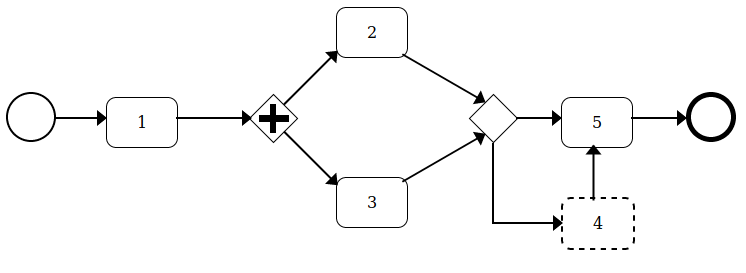
\includegraphics[width=\textwidth]{img/bad_modeling/corrected_model}
	\caption{Pataisyto veiklos modelio pavyzdys}
	\label{img:corrected_model}
\end{figure}
\begin{figure}[H]
	\centering
	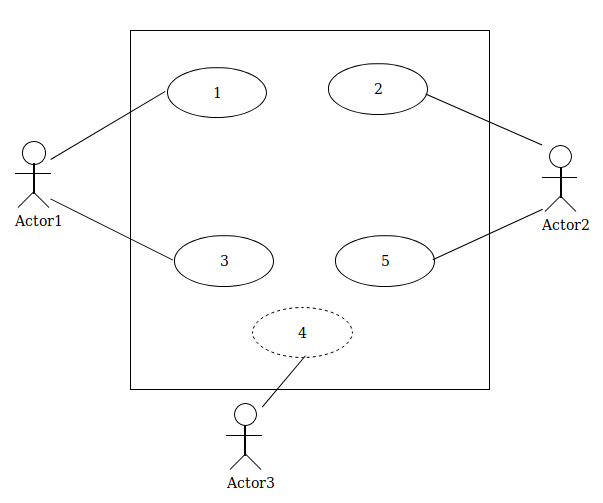
\includegraphics[width=15cm]{img/bad_modeling/corrected_model_use_cases}
	\caption{Vartojimo atvejų diagramos sukurtos pagal \ref{img:corrected_model} pav. pavyzdys}
	\label{img:corrected_model_use_cases}
\end{figure}

Sumažinti klaidų kiekį galima užrašant turimus duomenis ir automatiškai generuojant modelius. Generavimo įrankis galėtų patikrinti ar įvesties duomenys atitinka keliamus reikalavimus. Taip bus parodyti netikslumai ir analitikas galės pakoreguoti modelį.

Šio darbo tikslas – sukurti algoritmą \BPMN{} modelio transformacijai į užduočių diagramas ir įgyvendinti programos prototipą. Užduočių diagramos yra svarbi reikalavimų inžinerijos dalis, kadangi ji apibrėžia naudotojo reikalavimus. Įmonės dažniausiai žino kaip ir kokias veiklas jos vykdo. Verslo procesą galima apibrėžti \BPMN{} diagramomis. Bet ne viską, kas yra \BPMN{} modelyje, galima perkelti į užduočių diagramą, todėl darbe bus apibrėžtas modifikuotas \BPMN{} modelis, kuriame bus vaizduojama tik algoritmui aktuali informacija. Taip pat gali tekti pridėti papildomų atributų, kurie padės pasiekti tikslesnius rezultatus. Čia bus tiriamas \BPMN{} modelio transformacijos į užduočių diagramas algoritmas.

Siekiami rezultatai yra:
\begin{enumerate}
	\item Algoritmas galintis transformuoti \BPMN{} modelį į užduočių diagramą(angl. Use case diagram).
	\item Programa demonstruojanti algoritmo veikimą.
\end{enumerate}

\section{Veiklos srities modeliavimo metodai ir kalbos}
\subsection{BPMN diagrama} \label{section:bpmn}
Norint standartizuoti verslo modelių atvaizdavimą 2004 metais organizacija BPMI išleido \BPMN{} 1.0 specifikaciją. Ji leido tiek vaizduoti esamus, tiek apsikeisti kuriamų procesų reikalavimais. \BPMN{} greitai išpopuliarėjo tarp vadybininkų, verslo analitikų ir programuotojų, nes pasiūlė pažįstamą verslo procesų atvaizdavimą ir turėjo matematinį pagrindą. Vėliau BPMI susijungė su \OMG{} ir 2013 metais buvo išleista \BPMN{} 2.0 versija, kurioje \BPMN{} įgavo geresnį skaitomumą, lankstumą ir išplečiamumą.

\subsubsection{BPMN apimtis}
\BPMN{} specifikacija standartizuoja verslo procesų modelį, jų atvaizdavimo būdą ir duomenų apsikeitimo formatą perduoti tiek modelį, tiek jo atvaizdavimą. Sutelkti dėmesiui į skirtingas proceso dalis pateikiami procesų ir choreografijos submodeliai. Bendradarbiavimo submodelis, į save įtraukiantis kitus, gali būti naudojamas pateikti iš karto viskam. Specifikacijos apimtis yra verslo procesai taigi dalykai kaip strategija, duomenų struktūros, resursai, taisyklės ir įstatymai neįeina į ją.

\subsubsection{BPMN komponentai} \label{section:bpmn_components}
\BPMN{} specifikacija leidžia atvaizduoti gana nemažai verslo proceso atributų \cite{bpmnFormal}. Specifikacijoje jie yra suskirstyti į pagrindinius ir išvestinius. Toliau pateikiami pagrindiniai \BPMN{} komponentai.

\begin{figure}[H]
	\centering
	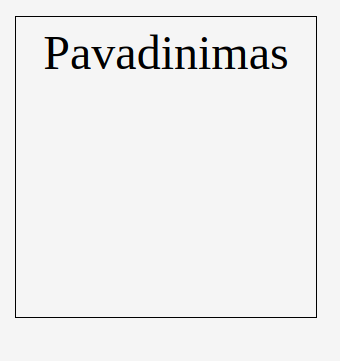
\includegraphics[width=5cm]{img/bpm-components/pool}
	\caption{Juostos žymuo}
	\label{img:bpm_components_pool}
\end{figure}

Juosta (pool) žymi diagramos dalyvį. Šio komponento paskirtis yra parodyti už kokias veiklas ir koks vykdytojas yra atsakingas. Juosta gali būti skaidoma smulkiau norint konkrečiau nurodyti vykdytojų grupes ir jų pareigas, tuomet ji gali būti vadinama linija (lane). Juosta žymima apibraukiant tam tikrą sritį (\ref{img:bpm_components_pool} pav.). Viduje yra vieta komponentams už kurių atlikimą atsakingas dalyvis.

\begin{figure}[H]
	\centering
	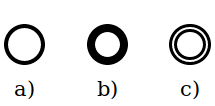
\includegraphics[width=5cm]{img/bpm-components/event_types}
	\caption{Įvykio žymuo}
	\label{img:bpm_event_types}
\end{figure}

Įvykis (event) žymi, kad įvyko kažkas, kas įtakojo proceso būseną. Šis komponentas dažniausiai turi priežastį (trigger) dėl ko jis įvyko ir pasekmes (result). Specifikacijoje įvykiai skirstomi į tris tipus: pradžios (\ref{img:bpm_event_types} pav. a), pabaigos (\ref{img:bpm_event_types} pav. b) ir tarpinius (\ref{img:bpm_event_types} pav. c). Žymėjimas yra tuščias apskritimas (\ref{img:bpm_event_types} pav.), viduje paliekant vietos tipo konkretizavimui.

\begin{figure}[H]
	\centering
	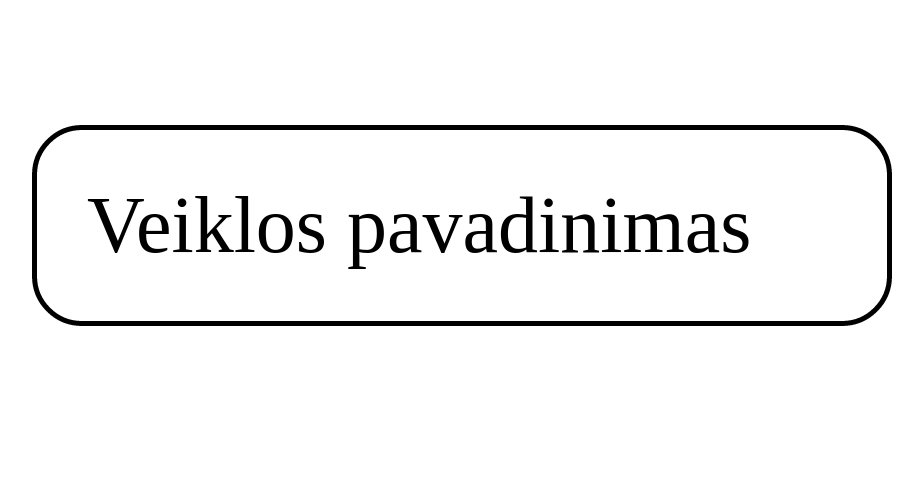
\includegraphics[width=5cm]{img/bpm-components/activity}
	\caption{Veiklos žymuo}
	\label{img:bpm_components_activity}
\end{figure}

Veikla (Activity) yra darbas atliekamas organizacijos procesuose. Ji gali būti atominė ir turėti tik pavadinimą arba  skaidoma labiau, tokiu būdu tapdama subprocesu. Visais atvejais žymėjimas yra stačiakampis su užapvalintais kampais (\ref{img:bpm_components_activity} pav.).

\begin{figure}[H]
	\centering
	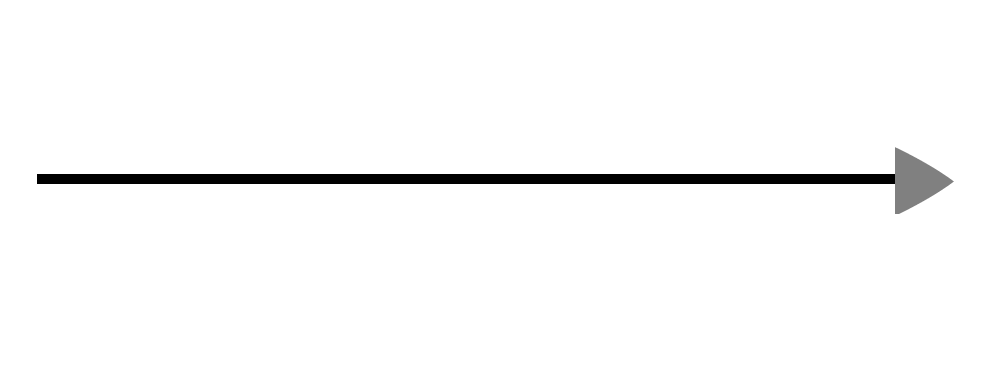
\includegraphics[width=5cm]{img/bpm-components/transition}
	\caption{Sekos srauto žymuo}
	\label{img:bpm_components_sequence_flow}
\end{figure}

Sekos srautas (Sequence Flow) žymi veiklų seką. Jeigu nenurodyta lygiagretumo veiklos modelyje vykdomos iš eilės. Šis komponentas parodo kokia tvarka tai vyks. Jį galima apibūdinti kaip grafo su kryptimis briauna, kryptis parodo kuri veikla turi būti įvykdyta vėliau. Sekos srautas žymimas solidžia linija ir užpildyto trikampio formos rodykle parodančia kryptį (\ref{img:bpm_components_sequence_flow} pav.).

\begin{figure}[H]
	\centering
	
\includegraphics[width=5cm]{img/bpm-components/gateway}
	\caption{Sprendimo žymuo}
	\label{img:bpm_components_gateway}
\end{figure}

Sprendimas (gateway) gali būti įterptas sekos srautuose tarp veiklų. Jis žymi srautų išsišakojimą arba susijungimą. Šis komponentas parodo, kad priklausomai nuo konkretaus proceso būsenos bus vykdomos veiklos į kurias eina sekos srautai atitinkantys sprendimo sąlygas. Žymėjimas yra kvadratas pasuktas 45 laipsniu kampu (\ref{img:bpm_components_gateway} pav.). Viduje yra vieta sprendimo konkretizavimui.

\begin{figure}[H]
	\centering
	
\includegraphics[width=5cm]{img/bpm-components/data_object}
	\caption{Duomenų objekto žymuo}
	\label{img:bpm_components_data_object}
\end{figure}

Duomenų objektas (data Object) pateikia informaciją apie tai kokių duomenų reikalauja veiklos vykdytojas norėdamas ją atlikti ir kokie duomenys pagaminami po jos vykdymo. Komponentas gali žymėti tiek neskaidomus tiek sudėtinius duomenis. Jis vaizduojamas (\ref{img:bpm_components_data_object} pav.) kaip stačiakampis su nukirptu dešiniuoju viršutiniu kampu ir trikampiu prie jo (arba kaip stačiakampis lapas su užlenktu dešiniuoju viršutiniu kampu).

\begin{figure}[H]
	\centering
	
\includegraphics[width=5cm]{img/bpm-components/message}
	\caption{Pranešimo žymuo}
	\label{img:bpm_components_message}
\end{figure}

Pranešimas (message) žymi bendravimą tarp dalyviu. Šis komponentas skirtas apibrėžti perduodamai informacijai tarp jų. Vaizduojamas (\ref{img:bpm_components_message} pav.) stačiakampiu su trikampiu viduje (vokas).

\begin{figure}[H]
	\centering
	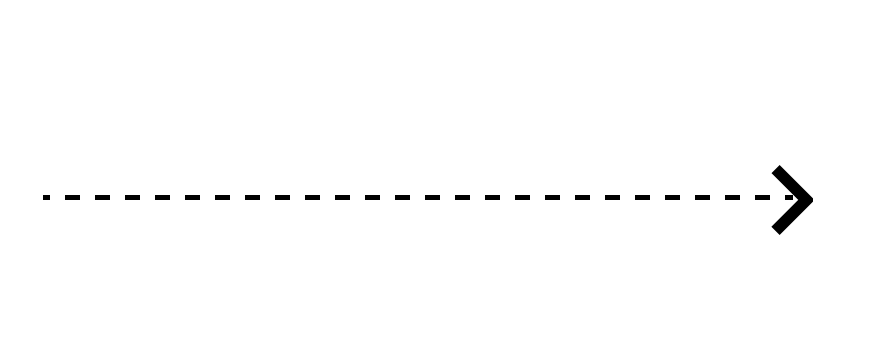
\includegraphics[width=5cm]{img/bpm-components/message_flow}
	\caption{Pranešimų srauto žymuo}
	\label{img:bpm_components_message_flow}
\end{figure}

Pranešimų srautas (Message flow) žymi duomenų perdavimą. Tai yra kryptinė grafo briauna, kuri jungia duomenų objektus ir žinutes su juos sukuriančiomis arba naudojančiomis veiklomis. Duomenų srautas į objektą ar žinutę rodo, kad tai yra veiklos išeiga, priešingu atveju tai yra veiklos įeiga, duomenys reikalingi jai įvykdyti. Vaizduojama (\ref{img:bpm_components_message} pav.) punktyrine linija su rodykle rodančia kryptį.

\begin{figure}[H]
	\centering
	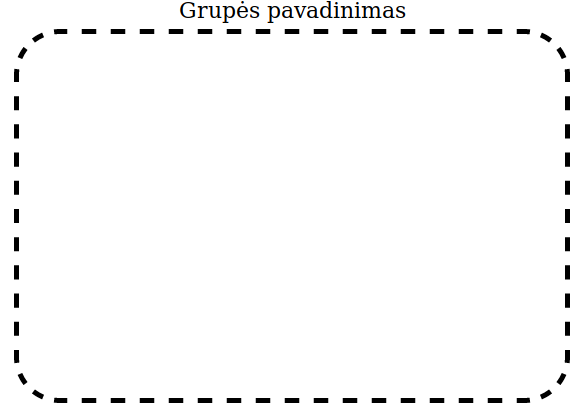
\includegraphics[width=5cm]{img/bpm-components/group}
	\caption{Grupės žymuo}
	\label{img:bpm_components_group}
\end{figure}

Grupė (group) skirta nurodyti modelio komponentų kategorijas. Ji neturi įtakos sekų ar duomenų srautams, o tik pasako kas priklauso tai pačiai kategorijai. Vaizdavimas diagramoje yra komponentų apibraukimas ir grupės pavadinimo nurodymas (\ref{img:bpm_components_group} pav.).

\begin{figure}[H]
	\centering
	
\includegraphics[width=5cm]{img/bpm-components/text_annotation}
	\caption{Komentaro žymuo}
	\label{img:bpm_components_text_annotation}
\end{figure}

Komentaras (text annotation) yra mechanizmas skirtas pateikti papildomai informacijai diagramos skaitytojams. Šis komponentas neįtakoja sekos ar duomenų srautų, o tik paaiškina kas ir kodėl vyksta. Žymimas skliaustu iš kairės komentaro teksto pusės (\ref{img:bpm_components_text_annotation} pav.).

\begin{figure}[H]
	\centering
	
\includegraphics[width=5cm]{img/bpm-components/association}
	\caption{Asociacijos žymuo}
	\label{img:bpm_components_text_association}
\end{figure}

Asociacija (association) skirta komentarams susieti su modelio komponentais. Ji nurodo kuri diagramos dalis yra komentuojama. Asociacija vaizduojama punktyrine linija (\ref{img:bpm_components_text_association} pav.).

\subsubsection{BPMN komponentų tarpusavio ryšiai}
Norint modeliuoti verslo procesus vien komponentų nepakanka, taip pat reikia žinoti ir kaip jie sąveikauja tarpusavyje. Tarpusavio ryšius gana neblogai apibūdina metamodelis. Šiame darbe jis bus dažnai naudojamas tam tikslui. Skyriuje \ref{section:bpmn_components} aprašytų komponentų sąveiką galima pavaizduoti (\ref{img:bpmn_metamodel} pav.) metamodeliu.

\begin{figure}[H]
	\centering
	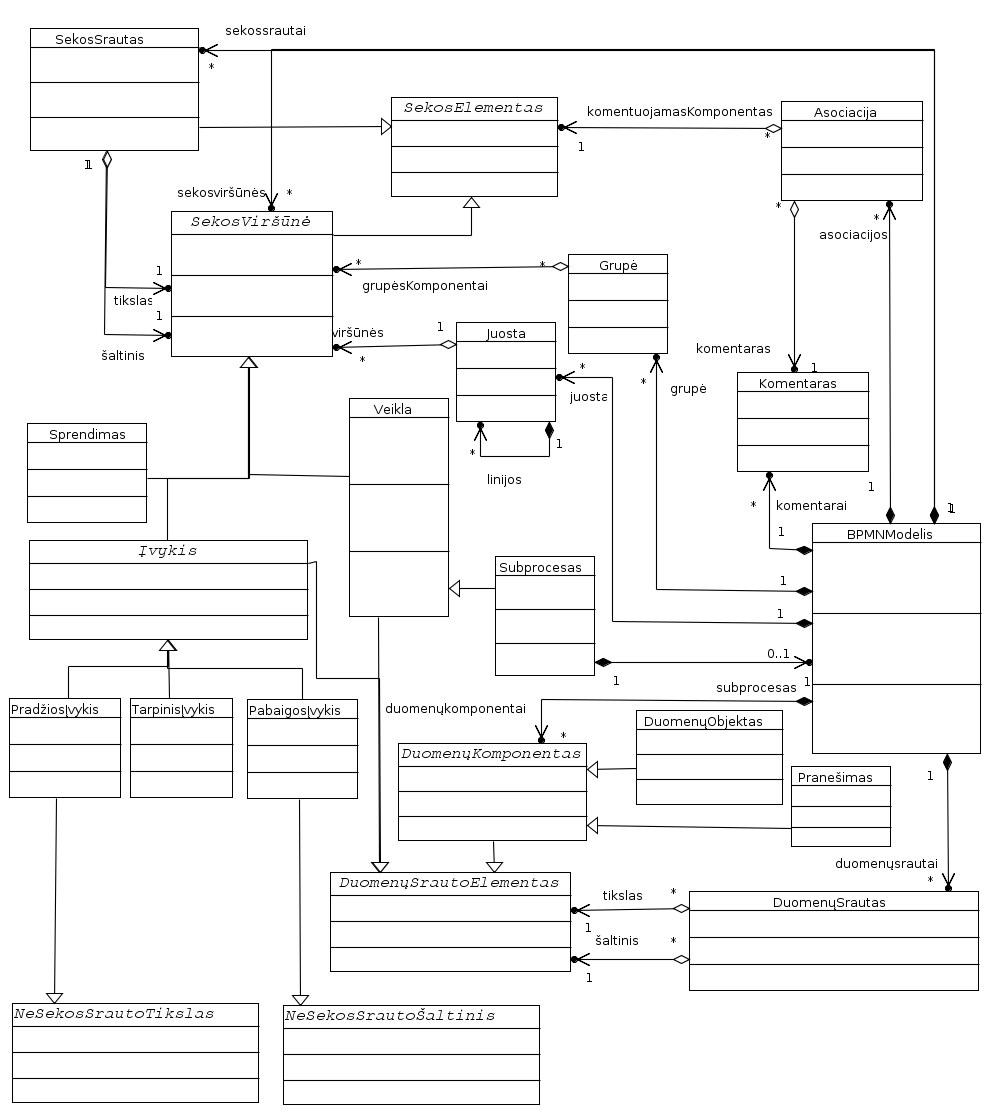
\includegraphics[width=\textwidth]{sections/modeling_methods_and_languages/img/bpmn_metamodel}
	\caption{\BPMN{} pagrindinių komponentų metamodelis}
	\label{img:bpmn_metamodel}
\end{figure}

Šiame metamodelyje tipas BPMNModelis yra šakninis komponentas. Jis savyje laiko
sekos viršūnes, sekos srautus, juostas, grupes, duomenų komponentus, duomenų
srautus, komentarus ir asociacijas. Komponentus metamodelyje galima suskirstyti
į tris grupes: sekos komponentus, duomenų komponentus ir komentavimo komponentus.
Sekos komponentams priklauso SekosElemento tipų hierarchija, duomenų
komponentams priklauso DuomenųKomponento hierarchija ir DuomenųSrautas,
komentavimui priklauso Komentaras ir Asociacija. Taigi galima iš eilės
apibūdinti šias grupes iš kurių susideda \BPMN{} modelis.

Sekos viršūnė yra abstrakcija nurodanti, kad tai yra komponentai jungiami
sekos srautais, tokie kaip veikla, sprendimas ir įvykio subtipai. Įvykis yra
abstraktus tipas nes modelyje būna kurie nors iš jo subtipų. Sekos srautas turi
vieną šaltinį ir vieną tikslą. Autorius įveda 2 abstrakcijas: ne sekos srauto
šaltinis ir ne sekos srauto tikslas, kad parodyti \BPMN{} apribojimus, kurie
draudžia pabaigos įvykiui būti sekos srauto šaltiniu, o pradžios įvykiui –
tikslu.  Grupės ir Juostos nurodo kurios sekos viršunės joms priklauso.
Juosta dar gali turėti linijų. Metamodelyje taip pat parodoma, kad Veikla gali
būti subprocesas, tokiu būdu savyje laikydama kitą procesą. Duomenų srauto
elementas yra autoriaus įvesta abstrakcija parodanti, kad jo subtipai gali
būti jungiami duomenų srautais. Įvesta abstrakcija duomenų komponentas norint
apibendrinti praneŠimą ir duomenų objektą. Komentaras jungiamas Asociacija ir
gali komentuoti sekos komponentus.

\subsection{Veiklos modeliavimas}

Veiklos modeliavimo metodologijas galima suskirstyti pagal savybes kuriomis jos
pasižymi. Šiuo atveju jos skirstomos pagal tai, kaip naudoja žinias
%ir pagal veiklos stebėjimo padėtį.
Toks suskirstymas parodys kaip sumodeliuoti daugiau
naudingos informacijos ir kodėl šiame darbe naudojamas detalizuotas grandinės
vertės modelis (\DVCM{}).

\begin{figure}[H]
	\centering
	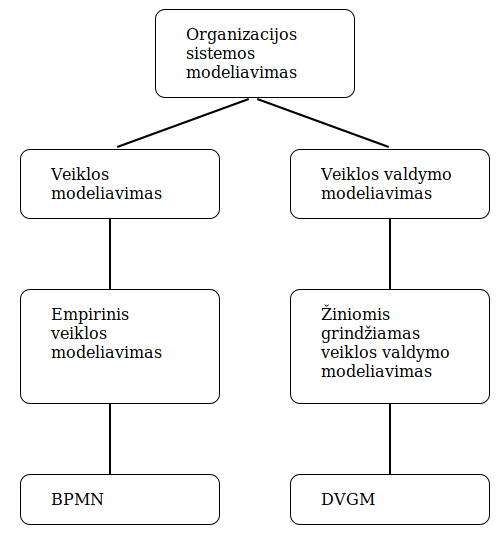
\includegraphics[width=10cm]{./sections/modeling_methods_and_languages/img/business_system_modeling}
	\caption{Veiklos modeliavimo požymiai pagal žinių naudojimą}
	\label{img:business_system_modeling}
\end{figure}

Skirstant veiklos modeliavimo metodus pagal žinių naudojimą galima pastebėti dvi
šakas (\ref{img:business_system_modeling} pav.). Pirmoje veikla
modeliuojama naudojant patirtį iš anksčiau stebėtų veiklų, tokiu atveju
analitikas sudaro modelį, kuris jo manymu bus teisingas. Prie tokių metodologijų
galima priskirti \BPMN{} . Antroje šakoje veiklos valdymas modeliuojamas
naudojant žinias apie tai kokį modelį reikia sudaryti. Šiuo atveju yra paimamas
teorijoje aprašytas modelis ir veiklos organizuojamos pagal jį. Tuo pasižymi
\DVCM{}.


%Pagal veiklos stebėjimo padėtį metodologijas galima suskirstyti į išorinio ir
%vidinio modeliavimo. Šie būdai parodo veiklą skirtingu detalumu. Modeliuojant
%išoriniu būdu parodomos veiklos naudojimas iš išorės.


\subsection{Detalizuotas vertės grandinės modelis – DVGM} \label{section:dvcm}

\BPMN{} modelyje galima pastebėti organizacijos valdymo veiklų supratimo neapibrėžtumus \cite{bpmnPorterModel}. Taip yra todėl, kad empirinio modeliavimo metodai neparodo informacijos arba resursų transformavimo priežasčių. Tačiau įmonę galima analizuoti ir transakcinių darbų sekų modelio (\ref{img:pdca} pav.) požiūriu, tokiu būdu organizuojant veiklą kaip teoriškai teisingą.

\begin{figure}[H]
	\centering
	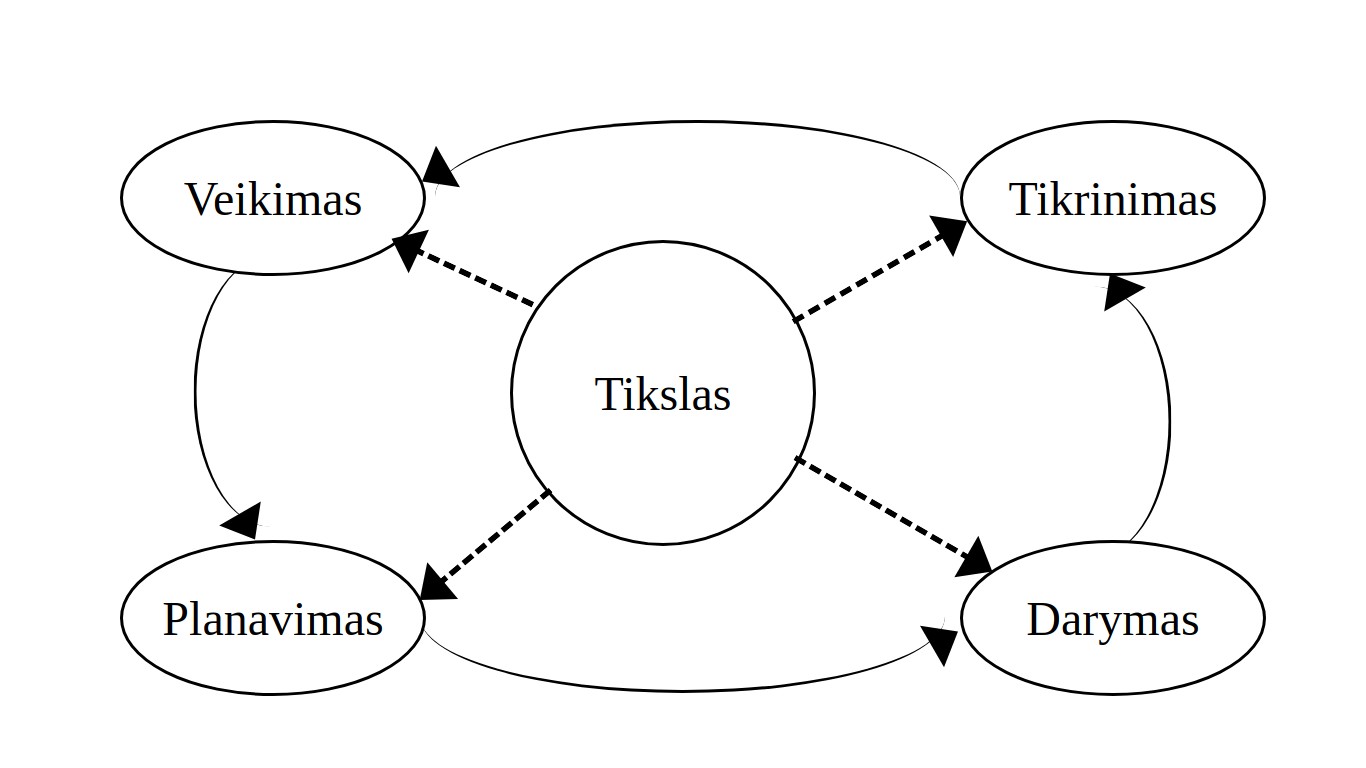
\includegraphics[width=10cm]{img/pdca}
	\caption{Transakcinių darbų sekų modelio pavyzdys}
	\label{img:pdca}
\end{figure}

%TODO: show goles in diagram
\begin{figure}[H]
	\centering
	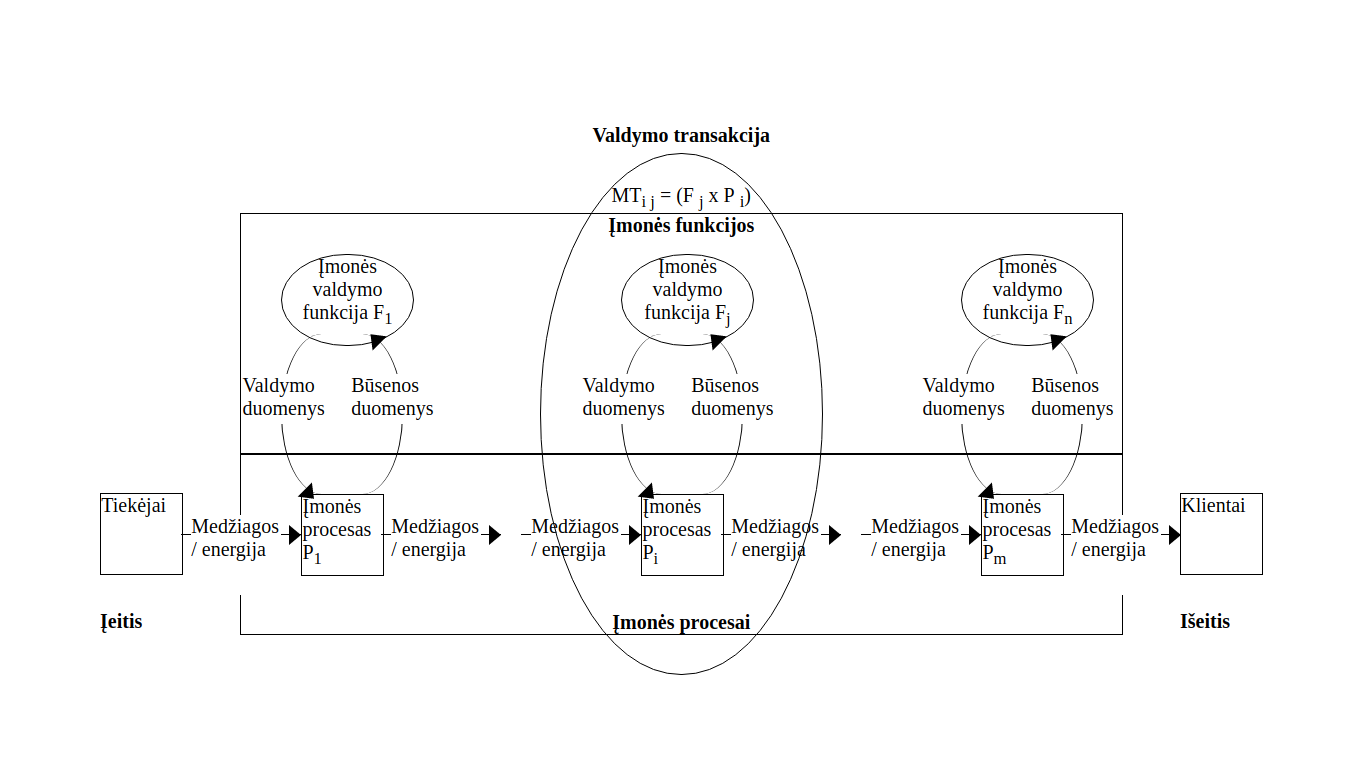
\includegraphics[width=\textwidth]{img/detalized_porter_vcm}
	\caption{Detalizuotas M. Porterio vertės grandinės modelis}
	\label{img:detalized_porter_vcm}
\end{figure}

Darbe organizacijos procesas bus nagrinėjamas kaip transakcijų visuma. Materialios
veiklos atskiriamos nuo valdymo veiklų. $P_i$ žymi veiklos procesą, kuris
transformuoja žaliavas, medžiagas, energiją ir formuoja materialią išeigą.
$F_j$ yra veiklos valdymo funkcija, informacijos (duomenų, žinių) transformavimo
veikla, būtina valdant procesą $P_i$. Modelis yra suskirstytas į valdymo
transakcijas $ MT_{ij} = F_j \times P_i$. Tokiu būdu pateikiama daugiau
informacijos apie įmonę. Diagrama bus vaizduojama kaip detalizuotas M.
Porterio vertės grandinės modelis (\ref{img:detalized_porter_vcm} pav).

Valdymo funkcija $F_j$ gali būti suskaidyta smulkiau.
(\ref{img:splitted_management_function} pav.) parodytas pavyzdys kai $F_j$
susideda iš smulkesnių dalių $F_{j1}$, $F_{j2}$ ir $F_{j3}$. Kartu visa tai
suteikia veiklos procesui $P_i$ valdymo duomenis kuriuos jis panaudoja vykdymui.
Vėliau grąžinami būsenos duomenys, jie panaudojami valdymo funkcijoje ir ciklas
kartojasi.

\begin{figure}[H]
	\centering
	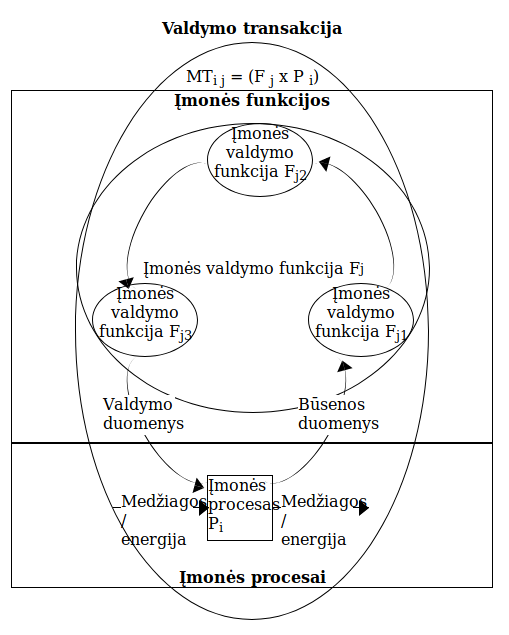
\includegraphics[width=7cm]{img/splitted_management_function}
	\caption{Valdymo funkcijos $F_j$ išskaidymo pavyzdys}
	\label{img:splitted_management_function}
\end{figure}


\subsubsection{DVGM apimtis}

Detalizuotas vertės grandinės modelis leidžia modeliuoti organizacijos veikimą kaip
transakcijų visumą. Jis atskiria vadybos veiklas nuo produkcijos veiklų.
Parodomi valdymo informacijos ciklai, kurie kontroliuoja produkcijos veiklą ir
padeda siekti organizacijos užsibrėžtų tikslų. Taip pat parodomi informacijos srautų
tipai, produkcijos veiklų įeigos ir išeigos tipai. Visa tai leidžia suprasti
kodėl įmonėje egzistuoja viena ar kita valdymo transakcija ir kaip jos įtakoja
organizacijos tikslų pasiekimą.

\subsubsection{DVGM komponentai}

Pateikiami pagrindiniai \DVCM{} komponentai. Jie leidžia veiklą modeliuoti kaip transakcinių darbų seką, kurioje procesai yra atskirti nuo valdymo funkcijų.

\begin{figure}[H]
	\centering
	
\includegraphics[height=2cm]{img/dvcm_components/management_function}
	\caption{Valdymo funkcijos žymuo}
	\label{img:dvcm_components_management_function}
\end{figure}

Valdymo funkcija (management function) darbas atliekamas organizacijoje, kuris prisideda į valdymo duomenų generavimą. Šio darbo įeiga paprastai savyje turi jo valdomo veiklos proceso proceso būseną. Atlikus darbą generuojami valdymo duomenys. Žymimas ovalu viduje paliekant vietos pavadinimui (\ref{img:dvcm_components_management_function} pav.).

\begin{figure}[H]
	\centering
	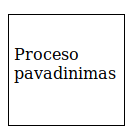
\includegraphics[height=2cm]{img/dvcm_components/process}
	\caption{Veiklos proceso žymuo}
	\label{img:dvcm_components_process}
\end{figure}

Veiklos procesas arba tiesiog procesas (process) yra darbas atliekamas organizacijoje, kuris tiesiogiai prisideda prie organizacijos gaminamos išeigos
sukūrimo. Šis komponentas valdomas valdymo funkcijų per valdymo transakcijose keliaujančius duomenis. Joms, atlikęs darbą, per interakcijų sekos srautus jis pateikia savo būsenos duomenis ir gauna valdymo duomenis. Žymimas stačiakampiu viduje paliekant vietos pavadinimui (\ref{img:dvcm_components_process} pav.).

\begin{figure}[H]
	\centering
	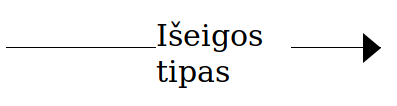
\includegraphics[height=1cm]{img/dvcm_components/sequence_flow}
	\caption{Interakcijų sekos srauto žymuo}
	\label{img:dvcm_components_sequence_flow}
\end{figure}

Interakcijų sekos srautas (interactions sequence flow) parodo valdymo funkcijų ir veiklos procesų seką, taip pat kas pagaminama atliekant darbus. Kadangi organizacijos veikla vaizduojama ciklais vieno darbo išeiga tampa kito įeiga. Šis komponentas vaizduojamas solidžia linija su užpildyto trikampio formos rodykle
gale ir išeigos (kuri tampa įeiga) tipo vardu prie pavaizduotos linijos (\ref{img:dvcm_components_sequence_flow} pav.).

\begin{figure}[H]
	\centering
	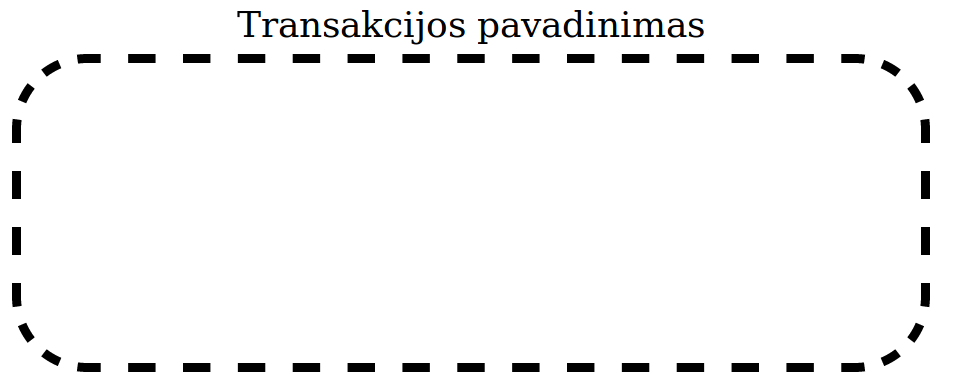
\includegraphics[height=2cm]{img/dvcm_components/management_transaction}
	\caption{Valdymo transakcijos žymuo}
	\label{img:dvcm_components_management_transaction}
\end{figure}

Valdymo transakcija (management transaction) parodo, kaip valdymo funkcijos kontroliuoja veiklos procesą. Šis komponentas žymi valdymo duomenų transformacijų ciklą. Jis vaizduojamas punktyrine linija apibraukiant transakcijai priklausantį veiklos procesą ir valdymo funkciją bei parašant transakcijos pavadinimą
(\ref{img:dvcm_components_management_transaction} pav.).

\subsubsection{DVGM komponentų tarpusavio ryšiai}

\DVCM{} komponentų tarpusavio ryšiai pavaizduoti metamodeliu (\ref{img:dvcm_metamodel} pav.). Šakninis komponentas DVGM savyje laiko valdymo transakcijas, interakcijų sekos srautus ir veiklas. Veiklos jungiamos interakcijų sekos srautais, jie taip pat nurodo kokią išeigą šiai interakcijai generuoja veikla. Veiklos skirstomos į veiklos procesus ir valdymo funkcijas. Valdymo transakcija turi nuoroda į procesą ir jį valdančią funkciją, kuri gali susidaryti iš smulkesnių dalių, taip pat sujungtų interakcijų srautais.

\begin{figure}[H]
	\centering
	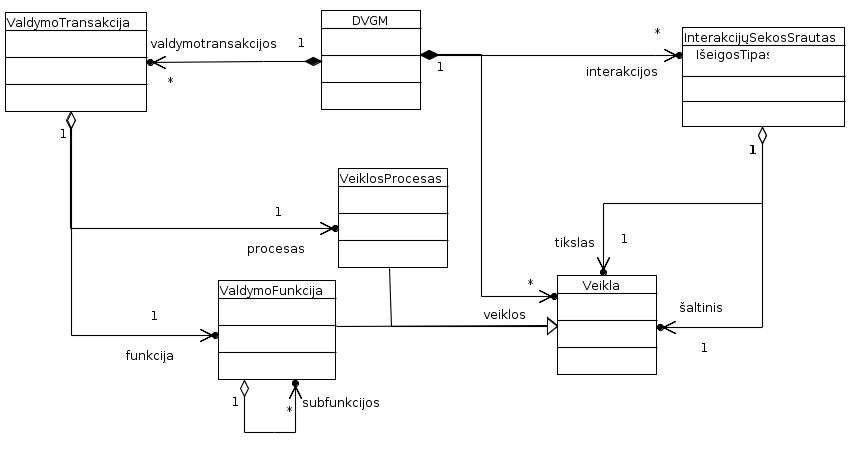
\includegraphics[width=\textwidth]{sections/modeling_methods_and_languages/img/dvcm_metamodel}
	\caption{\DVCM{} metamodelis}
	\label{img:dvcm_metamodel}
\end{figure}


\subsubsection{DVGM kaip BPMN praplėtimas}

\DVCM{} modelį galima apibrėžti ir kaip \BPMN{} praplėtimą. Paveikslas \ref{img:bpmn_extension_metamodel} vaizduoja tokį praplėtimo pavyzdį, tai bus įvesties duomenų formatas kuriamam algoritmui. Tokiu būdu apibrėžtą modelį galima nagrinėti kaip \BPMN{}.

\begin{figure}[H]
	\centering
	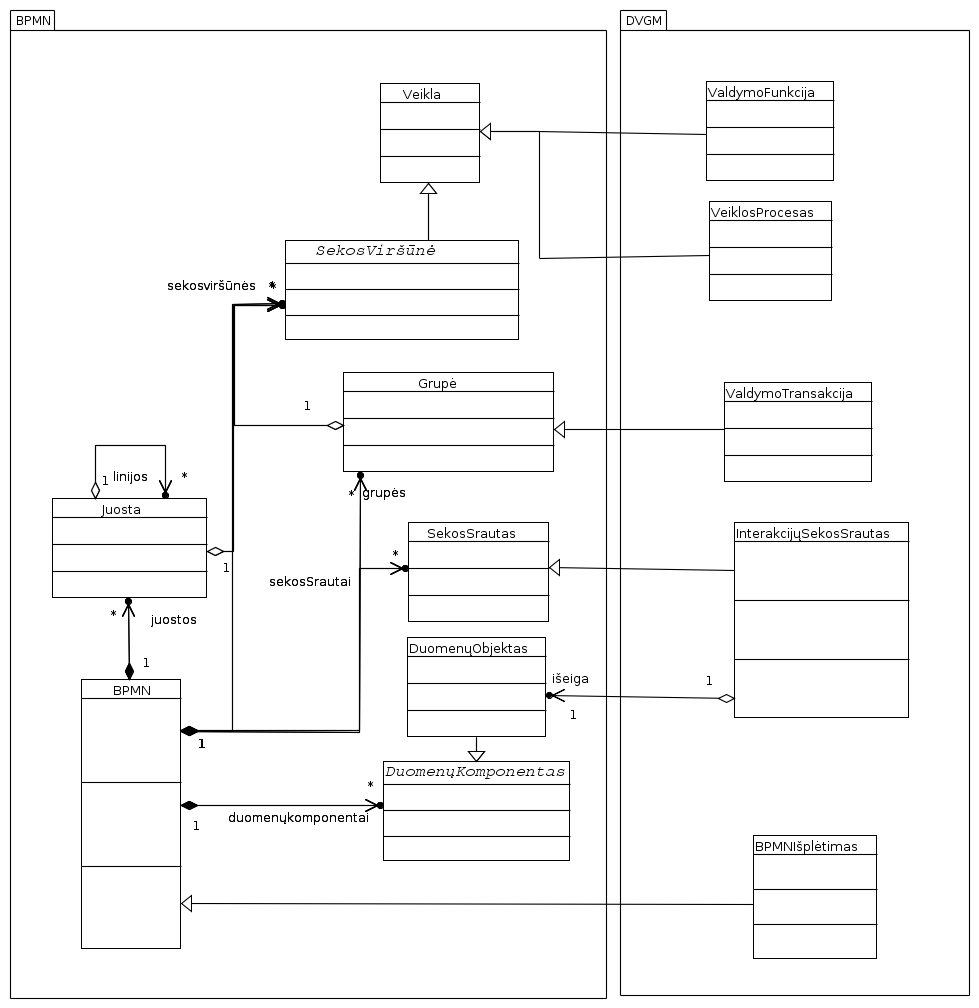
\includegraphics[width=\textwidth]{sections/modeling_methods_and_languages/img/bpmn_extension_metamodel}
	\caption{\DVCM{} kaip \BPMN{} praplėtimo metamodelis}
	\label{img:bpmn_extension_metamodel}
\end{figure}

\ref{img:bpmn_extension_metamodel} paveiksle \BPMN{} komponentai vaizduojami iš kairės, iš dešinės yra komponentai išplečiantys modelį. Veikla išplečiama valdymo funkcija ir veiklos procesu. Valdymo transakcija yra grupė, o interakcijų srautas rodo veiklų sekos srautą ir jų perduodamus duomenis. Visa Tai sudaro \BPMN{} išplėtimą.

\subsection{Užduočių diagrama}

1992 metais Ivar Jacobson apibrėžė metodologiją specifikuoti vartojimo atvejus \cite{Jacobson1992}. Jis pateikė būdą apibrėžti atvejus tiek tekstu (\ref{tab:text_use_cases_login} lentelė), tiek diagrama (\ref{img:use_cases_login} pav.). Tarp programų sistemų kūrėjų ši metodologija išpopuliarėjo kaip funkcinių reikalavimų apibrėžimo technika. \OMG{} savo specifikacijose \UML{} \cite{omgUmlFormal} ir \SysML{} \cite{OMGSysML} standartizuoja vartojimo atvejų modelį ir priskiria jį prie elgsenos apibūdinimo diagramų. 2011 metais Ivar Jacobson paskelbė užduočių modelio 2.0 versiją \cite{jacobson2011usecase}, kuri pritaikyta prie judrių metodologijų projektų įgyvendinimo.

\begin{center}
    \begin{longtable}{|p{\textwidth}|}
    \caption{Tekstinio naudojimo atvejo pavyzdys}
	\label{tab:text_use_cases_login}
	\\ \hline
    \begin{tabular}{@{}p{3.5cm}p{12cm}}
    	\\
    	\textbf{ID} & NA1
    	\\
    	\textbf{Pavadinimas} & Registruoto naudotojo autentifikavimas
    	\\
    \end{tabular}
    \\
    \textbf{Aktoriai}
    \begin{enumerate}
    	\item Registruotas naudotojas.
    	\item Išorinė autentifikavimo sistema.
	\end{enumerate}
    \\
    \textbf{Aprašas}

    Registruotas naudotojas autentifikuojamas sistemoje.

    \\
    \textbf{Prieš sąlygos}
    \begin{enumerate}
    	\item Naudotojas nėra autentifikuotas sistemoje.
	\end{enumerate}
    \\
    \textbf{Priežastys}
    \begin{enumerate}
    	\item Naudotojas pareikalavo būti autentifikuotas.
	\end{enumerate}
    \\
    \textbf{Po sąlygos}
    \begin{enumerate}
    	\item Naudotojas yra autentifikuotas sistemoje.
	\end{enumerate}
    \\
    \textbf{Pagrindinė užduočių seka}
    \begin{enumerate}
    	\item Sistema pateikia autentifikavimo variantus.
    	\item Naudotojas autentifikuojamas sistemos turimu autentifikavimo būdu.\label{seka:1_main_choose_autentification}
		  \item Sistema pateikia patvirtinimą, kad naudotojas autentifikuotas. \label{seka:1_main_success}
	\end{enumerate}
    \\
    \textbf{Alternatyvios užduočių sekos}
    \newlist{seka}{enumerate}{5}
	\setlist[seka]{label*=\arabic*.,leftmargin=2em}
	\setlist[seka,1]{label=\ref{seka:1_main_choose_autentification}.\arabic*.,leftmargin=2em}
	\begin{seka}
  		\item Naudotojas autentifikuojamas išorine autentifikavimo sistema.
	\end{seka}
    \\
    \textbf{Išimtinės užduočių sekos}
	\newlist{seka}{enumerate}{5}
	\setlist[seka]{label*=\arabic*.,leftmargin=2em}
	\setlist[seka,1]{label=*.\arabic*.,leftmargin=2em}
	\begin{seka}
  		\item Naudotojas atsisako autentifikavimo.
  		\begin{seka}
  			\item Naudotojas pateikia autentifikavimo atsisakymą.
  			\item Sistema nebereikalauja autentifikavimo duomenų.
  		\end{seka}
	\end{seka}
	\setlist[seka,1]{label=\ref{seka:1_main_success}.\arabic*.,leftmargin=2em}
	\begin{seka}
  		\item Nepavyksta autentifikuoti naudotojo pateiktais duomenimis.
  		\begin{seka}
  			\item Sistema naudotojui pateikia pranešimą apie tai, kad jis negali būti autentifikuotas pateiktais duomenimis.
  		\end{seka}
	\end{seka}
    \\
    \\ \hline
    \end{longtable}
\end{center}

Lentelėje nr. \ref{tab:text_use_cases_login} pavaizduotas autentifikavimo sistemoje  tekstinio naudojimo atvejo pavyzdys. Naudojimo atvejai paprastai turi identifikacijos numerį pagal kurį nurodomi reikalavimų specifikacijoje. Taip pat pavadinimą, kad būtų patogiau apie jį kalbėti. Išvardinami aktoriai dalyvaujantys vykdyme. Naudojimo atvejis trumpai ir aiškiai aprašomas. Nurodomos kokios aktualios sąlygos būna prieš vykdant, kas įtakojo vykdymą ir rezultatai. Tuomet išvardinamos užduotys reikalingos pasiekti rezultatui. Jeigu naudojimo atvejis gali būti įvykdytas keliais būdais, jie nurodomi alternatyviose užduočių sekose. Jeigu vykdant užduočių sekas gali atsitikti kažkas, dėl ko nepavyksta pasiekti sėkmingo rezultato sąlygų, tai nurodoma išimtinėse užduočių sekose.

\begin{figure}[H]
	\centering
	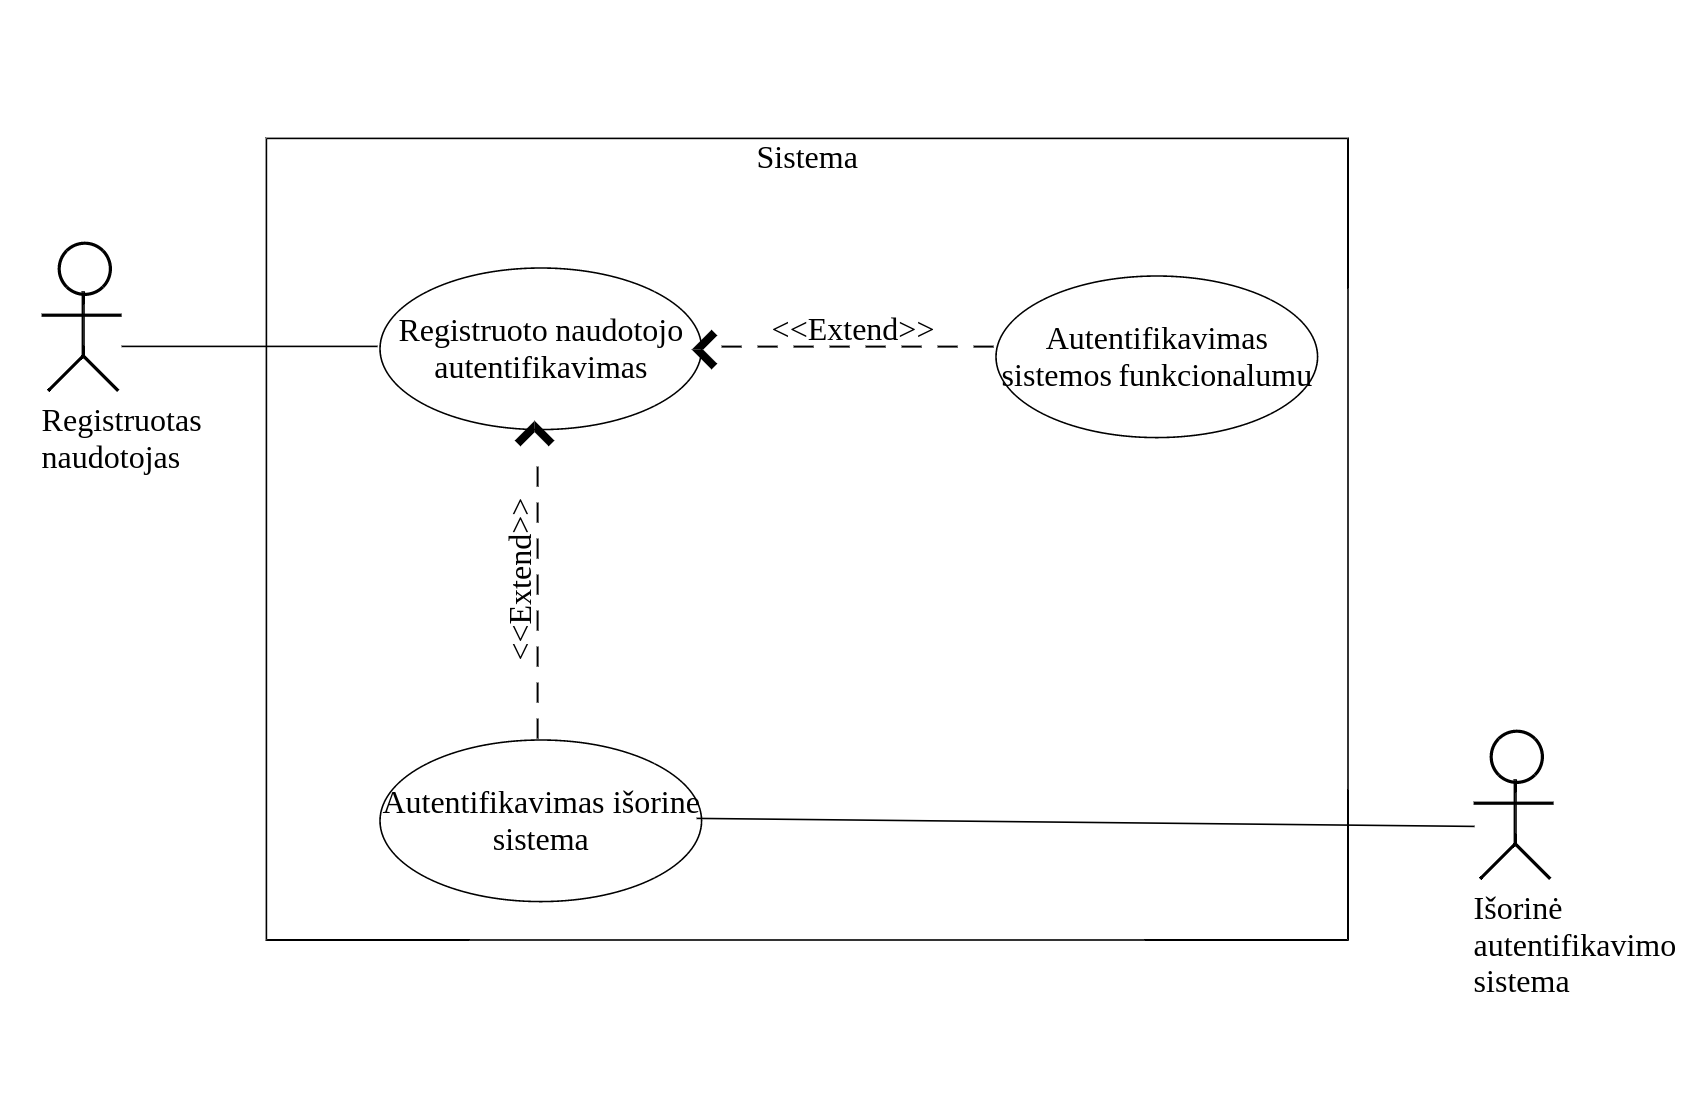
\includegraphics[height=8cm]{sections/modeling_methods_and_languages/img/use_cases_login}
	\caption{Užduočių diagrama pagal \ref{tab:text_use_cases_login} lentelę}
	\label{img:use_cases_login}
\end{figure}

Naudojimo atvejus galima atvaizduoti užduočių diagrama. \ref{img:use_cases_login} paveikslas vaizduoja \ref{tab:text_use_cases_login} lentelėje aprašytą naudojimo atvejo užduočių diagramą. Pagrindinė užduočių seka pavaizduota naudojimo atveju „Autentifikavimas sistemos funkcionalumu”,  alternatyvi – „Autentifikavimas išorine sistema”, išimtinės sekos nepavaizduotos.


\subsubsection{Užduočių diagramos apimtis}
Užduočių diagrama skirta apibūdinti kaip naudotojai siekia savo tikslų pasitelkdami sistemą. Ji parodo kokie yra funkciniai reikalavimai, naudotojų taksonomiją, duomenų srautus tarp naudotojų ir sistemos. Taip pat pateikia funkcijų hierarchijos modeliavimą ir leidžia jas suskaidyti (naudojant įtraukimo ryšį). Užduočių diagrama apibūdina funkcinius reikalavimus, ji nepateikia nei funkcijų atlikimo tvarkos, nei duomenų struktūrų naudojamų sistemoje.

\subsubsection{Užduočių diagramos komponentai} \label{section:use_cases_components}
Skirtingi šaltiniai pateikia kiek skirtingus komponentus ir jų apibrėžimus. Šiame darbe daugiausia taikomi \OMG{} standartuose pateikti apibrėžimai. Toliau bus pateikiami \UML{} standarte apibrėžtos užduočių diagramos komponentai.

\begin{figure}[H]
	\centering
	
\includegraphics[height=2cm]{img/use_case_components/actor}
	\caption{Aktoriaus žymuo}
	\label{img:use_case_components_actor}
\end{figure}

Aktorius (actor) žymi naudotojo rolę. Ją gali atlikti tiek žmogus, tiek išorinė programų sistema. Aktoriai sąveikauja su bendravimo kanalais prijungtais naudojimo atvejais. Šis komponentas žymimas žmogumi iš pagaliukų (\ref{img:use_case_components_actor} pav.).

\begin{figure}[H]
	\centering
	
\includegraphics[height=2cm]{img/use_case_components/use_case}
	\caption{Naudojimo atvejo žymuo}
	\label{img:use_case_components_use_case}
\end{figure}

Naudojimo atvejis (use case) žymi veiklų kurias atlikus gaunamas naudingas rezultatas aibę. Rezultatas gali būti naudingas tiek vykdytojui, tiek kitiems suinteresuotiems žmonėms. Šis komponentas vaizduojamas elipse (\ref{img:use_case_components_use_case} pav.),
naudojimo atvejo pavadinimas gali būti tiek elipsėje, tiek po ja.

\begin{figure}[H]
	\centering
	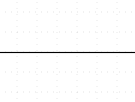
\includegraphics[width=5cm]{img/use_case_components/association}
	\caption{Bendravimo kanalo žymuo}
	\label{img:use_case_components_communication_path}
\end{figure}

Bendravimo kanalas (communication path) žymi sąveika tarp aktoriaus ir sistemos. Šis komponentas diagramoje jungia aktorių su naudojimo atveju, taip parodydamas, kad prieš atlikdamas veiklas (sistemos funkcijas) naudotojas pateikia įvestį o po jų atlikimo gaunamas rezultatas. Jeigu bendravimo kanalo ryšio su aktoriumi gausa yra daugiau nei 1 reiškia naudojimo atvejui atlikti reikalingi keli vykdytojai, jeigu bendravimo kanalo ryšio su naudojimo atveju gausa yra daugiau nei 1 reiškia aktorius gali atlikti tas pačias veiklas daugiau nei vieną kartą. Asosijacija žymima solidžia linija (\ref{img:use_case_components_communication_path} pav.).

\begin{figure}[H]
	\centering
	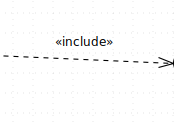
\includegraphics[height=2cm]{img/use_case_components/includes}
	\caption{Įtraukimo žymuo}
	\label{img:use_case_components_includes}
\end{figure}

Įtraukimas (includes) žymi naudojimo atvejo suskaidymą. Šis komponentas modeliuoja sąryši tarp dviejų vartojimo atvejų, taip parodydamas, kad įtraukiamo naudojimo atvejo veiklos yra atliekamos įtraukiančiame naudojimo atvejyje. Įtraukimą numatyta naudoti tuomet, kai tos pačios veiklos pasikartoja keliuose naudojimo atvejuose. Tos veiklos įdedamos į atskirą naudojimo atvejį ir prijungiamos šiuo ryšiu, tokiu būdu iškeliamas pasikartojantis funkcionalumas. Įtraukimas vaizduojamas punktyrine linija su rodykle  prie įtraukiamo naudojimo atvejo ir patikslinimu dvigubuose kampiniuose skliaustuose (\ref{img:use_case_components_includes} pav.).

\begin{figure}[H]
	\centering
	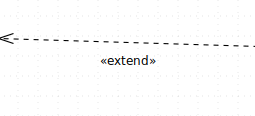
\includegraphics[height=2cm]{img/use_case_components/extend}
	\caption{Išplėtimo žymuo}
	\label{img:use_case_components_extends}
\end{figure}

Išplėtimas (extends) žymi, kad esant tam tikroms sąlygoms naudojimo atvejis įtraukia veiklas iš kitų naudojimo atvejų. Šis komponentas numatytas naudoti bendram funkcionalumui iškelti, bet kitaip nei ryšys „Įtraukia“, parodo, kad veiklos įtraukiamos ne visada. Jis vaizduojamas punktyrine linija su rodykle prie išplečiamo naudojimo atvejo ir patikslinimu dvigubuose kampiniuose skliaustuose (\ref{img:use_case_components_extends} pav.).

\begin{figure}[H]
	\centering
	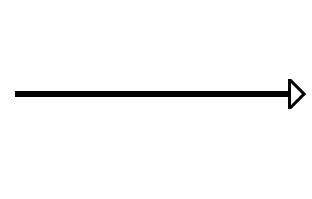
\includegraphics[height=2cm]{img/use_case_components/generalization}
	\caption{Apibendrinimo žymuo}
	\label{img:use_case_components_generalization}
\end{figure}

Apibendrinimas (generalization) žymi, kad elementas yra bendresnio elemento variantas. Nuo išplėtimo naudojimo atvejo apibendrinimas skiriasi tuo, kad pasakoma jog bent vienas iš apibendrinamų naudojimo atvejų funkcionalumų įtraukiamas į apibendrinančio naudojimo atvejo funkcionalumą. Žymimas solidžia linija su rodykle prie apibendrinamo naudojimo atvejo (\ref{img:use_case_components_generalization} pav.).

\subsubsection{Užduočių diagramos komponentų tarpusavio ryšiai}

Komponentų aprašytų \ref{section:use_cases_components} skyriuje tarpusavio ryšiai  pavaizduoti metamodeliu (\ref{img:use_cases_metamodel} pav.). Jis sudarytas pagal \UML{} ir \SysML{} standartuose pateiktą informaciją.

\begin{figure}[H]
	\centering
	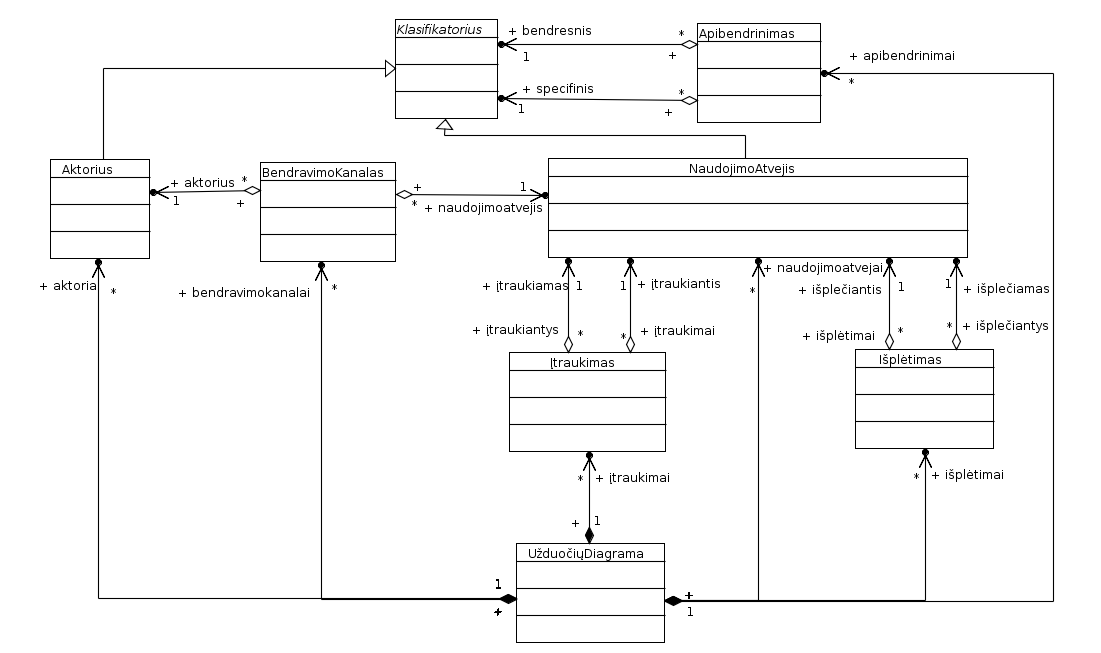
\includegraphics[width=\textwidth]{img/use_cases_metamodel}
	\caption{Užduočių diagramos metamodelis}
	\label{img:use_cases_metamodel}
\end{figure}

Užduočių diagrama yra paketas savyje laikantis aktorius, naudojimo atvejus, bendravimo kanalus, įtraukimus, išplėtimus ir apibendrinimus. Bendravimo kanalas jungia vieną aktorių su vienu naudojimo atveju. Įtraukimas yra ryšys tarp įtraukiamo ir įtraukiančio naudojimo atvejo. Išplėtimas jungia išplečiamą naudojimo atvejį su išplečiančiu. \UML{} modelis leidžia abstraktaus tipo klasifikatoriaus apibendrinimą. Aktorius ir naudojimo atvejis yra klasifikatoriaus subtipai, todėl gali būti apibendrinti.


\section{Veiklos modelių konvertavimas}
\subsection{UML diagramų transformavimo algoritmai} \label{section:main_use_cases_from_bpmn}
\subsection{ Algoritmas BPMN modeliui transformuoti į Užduočių diagramą} \label{section:use_cases_from_bpmn}
Literatųroje yra parašyta apie \textbf{vartojimo atvejų diagramos} išvedimą iš \BPMN{} modelio \cite{algUseCasesFromBpmn}. Straipsnyje aprašytas algoritmas atlieka (\ref{eq:use_cases_from_bpmn}) transformaciją. Imamas modifikuotas \BPMN{} modelis (\ref{eq:use_cases_from_bpmn:bpmn_elements}) ir tie \textbf{vartojimo atvejų diagramos} komponentai, kurie gali būti iš jo išvesti (\ref{eq:use_cases_from_bpmn:use_case_elements}). 
\begin{align}
&BPMNElements = \left\{Start,End,Role,Branch,Task,Transition\right\}; \label{eq:use_cases_from_bpmn:bpmn_elements} \\
\begin{split}
&UseCasesElements = \left\{Actor, Generalization, Association,Use Case,\right. \\
&\left. Include, Extension Point, Extend\right\}; \label{eq:use_cases_from_bpmn:use_case_elements}\\
\end{split} \\
&BPMN(BPMNModelElements) \Rightarrow UseCases(UseCasesElements); \label{eq:use_cases_from_bpmn}
\end{align}

Algoritmo autoriai pirmiausia siūlo surasti ryšius tarp modelių. Juostos atitinka aktorius. Užduotys tuo tarpu grupuojamos, kol nepasiekia maksimalaus skaičiaus vykdomų be pertraukos, priklausančių tai pačiai juostai ir pagaminančių rezultatą. Tokia grupė pavadinama žingsniu ir yra laikoma atitinkančia vartojimo atvejį.  Tuomet lieka surasti kaip dar galima būtų panaudoti informaciją, patikslinti ir suprastinti gautoms diagramoms.

Vėliau pristatomas algoritmas. Jis Pirmiausia sudėlioja užduotis į proceso žingsnius. Vėliau juostos tampa aktoriais, o žingsniai jose – vartojimo atvejais. Galiausiai pasikartojančios užduotis išimamos iš žingsnių ir prijungiamos bendravimo kanalu įtraukia arba išplečia pagal situaciją.

\subsection{Užduočių diagramos išvedimas iš BPMN modelio}

Šio darbo tikslas, algoritmas galintis gauti užduočių diagramas iš \BPMN{} modelio, bus kuriamas pagal \ref{section:use_cases_from_bpmn} skyriuje aprašytą algoritmo sukūrimo pavyzdį. Pirmiausia bus rasti ryšiai tarp diagramų, vėliau sukurtas būdas juos panaudoti, galiausiai panaudota likusi modelio informacija patikslinti ir suprastinti diagramoms.

Nuo anksčiau minėto algoritmo jis skirsis tuo, kad naudos \BPMN{} sukonstruota pagal \DVCM{} metodologiją kaip įvesties duomenis.  \ref{section:use_cases_from_bpmn} skyriuje aprašytas algoritmas įvestiems duomenims aprašyti siūlo modifikuotą \BPMN{} modelį ir užduočių diagramas sudaro vadovaudamasis empirinėmis taisyklėmis pasakančiomis kada geriau konstruoti užduotį. Šiame darbe kuriamas algoritmas užduotis konstruos remdamasis \DVCM{} apibrėžta veiklos organizavimo teorija. Tai leis tiksliau apibrėžti užduočių diagramos naudojimo atvejų tarpusavio ryšius. \ref{section:use_cases_from_bpmn} algoritmo autorių siūlomas būdas apibrėžti veiklos žingsnius atitinka \DVCM{} transakciją, tokiu būdu nereikia taikyti empirinių taisyklių ieškant žingsnio pradžios ir pabaigos.

\subsubsection{Ryšiai tarp BPMN ir užduočių diagramų} \label{section:relations_sd_bpmn}

Norint duomenis iš vieno modelio perkelti į kitą galima pasinaudoti ryšiais esančiais tarp jų.

\begin{center}
    \begin{longtable}{ | l | c |  c | c | c | c |}
    \caption{Ryšiai tarp \DVCM{} kaip \BPMN{} praplėtimo ir užduočių diagramų}
	\label{tab:relations_sd_bpmn}
    \\ \hline
     &
     %\begin{turn}{-90}
     Aktorius
     %\end{turn}
     &
     %\begin{turn}{-90}
     Vartojimo atvejis
     %\end{turn}
     &
     %\begin{turn}{-90}
     Bendravimo kanalas
     %\end{turn}
     &
     %\begin{turn}{-90}
     Įtraukia
     %\end{turn}
     &
     %\begin{turn}{-90}
     Išplečia
     %\end{turn}
     \\
    \hline
    Juosta & + & &  &  &  \\
    \hline
    Valdymo funkcija  & & + &  & + & + \\
    \hline
    Įmonės procesas  & + &  &  &  &  \\
    \hline
    Valdymo transakcija & & + & & + & + \\
    \hline
    Interakcijų sekos srautas  & &  & + & & \\
    \hline
    %Įvykis  & & & & & \\
    %\hline
    %Duomenų objektas  & & & & & \\
    %\hline
    %Pranešimų srautas  & & & & & \\
    %\hline
    %Sprendimas  & & & & & \\
    %\hline
    \end{longtable}
\end{center}

Iš juostos galima gauti Aktorius. Valdymo funkcija turi informacijos apie tai kokie vartojimo atvejai yra sistemoje ir kaip jie susiję vienas su kitu. Įmonės procesas taip pat yra aktoriai naudojantys sistemą. Valdymo transakcija yra vartojimo atvejis. Interakcijų sekos srautas parodo kokie duomenys keliauja bendravimo kanalais. Rasti ryšiai taip pat parodo kurie komponentai bus imami ir kurie gaunami. Taigi galima apibrėžti algoritmo įvesties ir išvesties duomenis.

\subsubsection{Ryšių tarp diagramų panaudojimas transformacijai}

Rasti ryšiai parodo į kokius \DVCM{} komponentus reikia žiūrėti išvedant užduočių diagramos dalis. Toliau peržiūrimi diagramos variantai ir sudėliojami konkretūs žingsniai kuriuos reikia atlikti. Galiausiai gaunamas pseudokodas (Pseudokodas \ref{lst:bpmn_to_uc_pseudocode}). Jo veikimas pažingsniui aprašomas, taip pat pavaizduotas (pav. \ref{img:algorythm_activity_diagram}).

\begin{figure}[H]
	\centering
	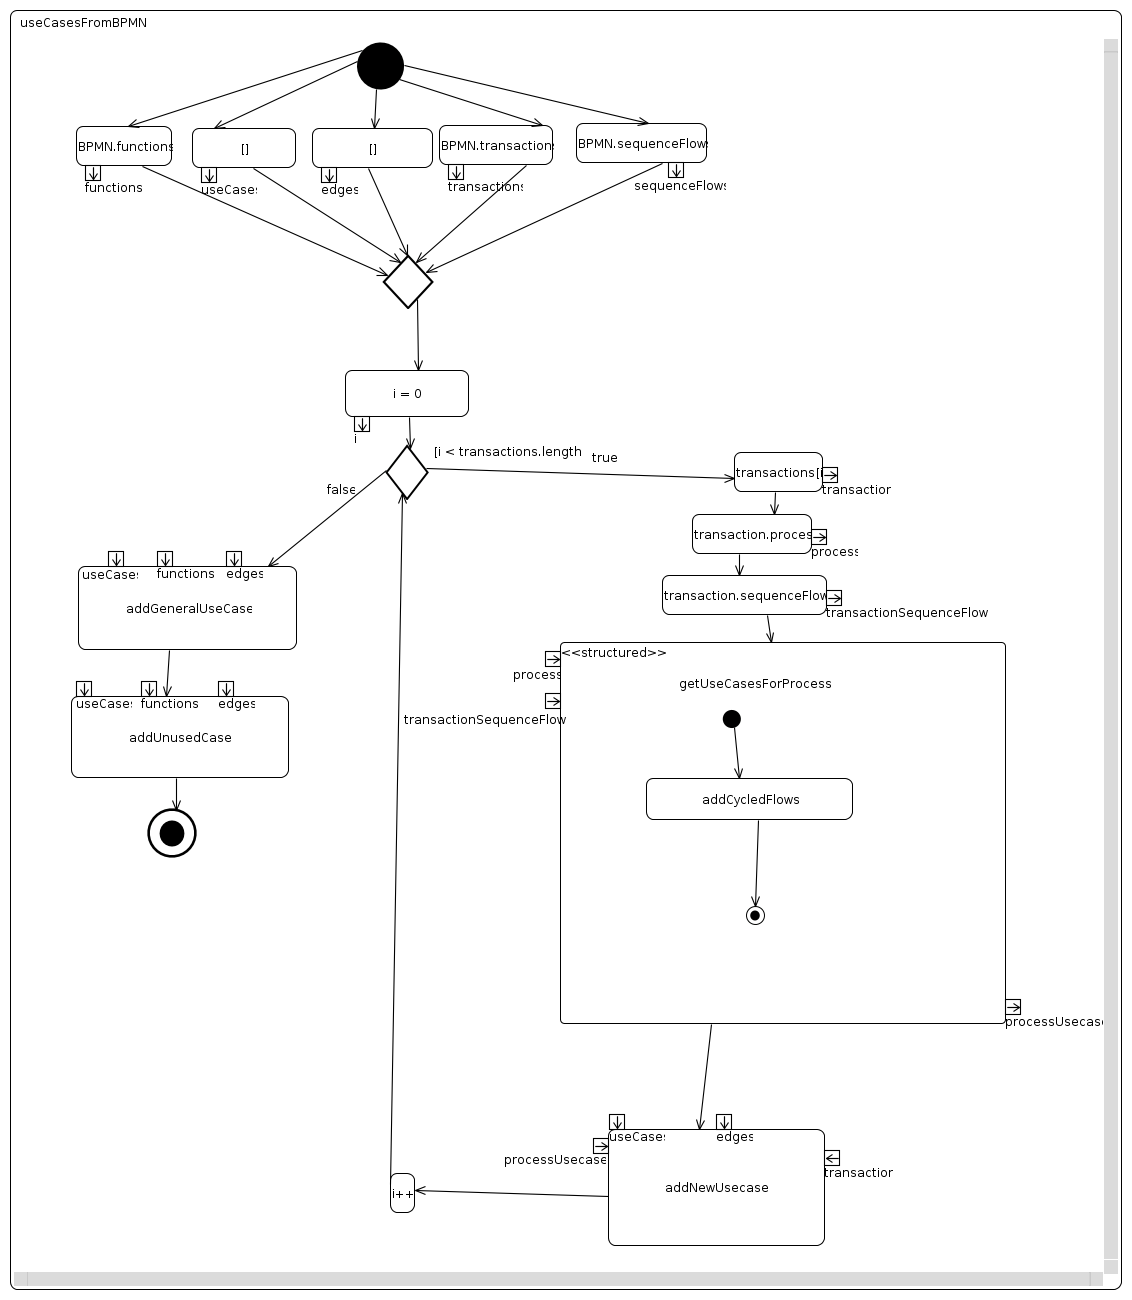
\includegraphics[scale=0.5]{img/algorythm-activity-diagram}
  \caption{Algoritmo diagrama}
	\label{img:algorythm_activity_diagram}
\end{figure}

\renewcommand{\lstlistingname}{Pseudokodas}% Listing -> Algorithm
\renewcommand{\lstlistlistingname}{Pseudokodo fragmentai}% List of Listings -> List of Algorithms
\begin{enumerate}
	\item Iškviečiama funkcija useCasesFromBPMN (Pseudokodas \ref{lst:bpmn_to_uc_pseudocode}) paduodant jai \BPMN{} modelį.

	\lstinputlisting[style=pseudocode, caption={\UML{} Užduočių diagramos gavimo iš \BPMN{} modelio algoritmo pseudokodas}, label={lst:bpmn_to_uc_pseudocode}]{algorythm-pseudocode/useCasesFromBPMN}

	\item Po duomenų inicializavimo pirmiausia imamas transakcijos procesas (eil. \ref{line:bpmn_to_uc_pseudocode_get_process}) ir gaunami sekos srautai jungiantys komponentus transakcijoje (eil. \ref{line:bpmn_to_uc_pseudocode_get_transactionSequenceFlows}).
	\item Vėliau sukuriami vartojimo atvejai apibrėžiantys proceso valdymą (eil. \ref{line:bpmn_to_uc_pseudocode_get_processUsecases}) funkcija getUseCasesForProcess (Pseudokodas  \ref{lst:bpmn_to_uc_pseudocode_getUseCasesForProcess}).

	\lstinputlisting[style=pseudocode, caption={Funkcija getUseCasesForProcess}, label={lst:bpmn_to_uc_pseudocode_getUseCasesForProcess}]{algorythm-pseudocode/getUseCasesForProcess}

	\item Joje randami sekos srautai išeinantys iš proceso (eil. \ref{line:bpmn_to_uc_pseudocode_getUseCasesForProcess_get_processFlows}) ir kiekvienam iš jų rekursijos būdu surandami ciklai su procesu funkcija addCycledFlows (Pseudokodas  \ref{lst:bpmn_to_uc_pseudocode_addCycledFlows}). Kiekvienam iš cikle esančių sekos srautų sukuriamas vartojimo atvejis (eil. \ref{line:bpmn_to_uc_pseudocode_getUseCasesForProcess_get_processUsecases_begin} - \ref{line:bpmn_to_uc_pseudocode_getUseCasesForProcess_get_processUsecases_end}). Jų kolekcija ir yra (Pseudokodas  \ref{lst:bpmn_to_uc_pseudocode_getUseCasesForProcess}) grąžinamas rezultatas.

	\lstinputlisting[style=pseudocode, caption={Funkcija addCycledFlows}, label={lst:bpmn_to_uc_pseudocode_addCycledFlows}]{algorythm-pseudocode/addCycledFlows}

Minėta Funkcija (Pseudokodas  \ref{lst:bpmn_to_uc_pseudocode_addCycledFlows}) pirmiausia patikrina ar jau nėra ciklo su procesu ir jei taip patvirtina, kad parametras currentPath turi savyje kelia į procesą (eil. \ref{line:bpmn_to_uc_pseudocode_addCycledFlows_isTargetProcess_begin} - \ref{line:bpmn_to_uc_pseudocode_addCycledFlows_isTargetProcess_end}). Jei kelias užsiciklino grąžinamas neigiamas atsakymas (eil. \ref{line:bpmn_to_uc_pseudocode_addCycledFlows_isGoingInCircles_begin} - \ref{line:bpmn_to_uc_pseudocode_addCycledFlows_isGoingInCircles_end}), tai reiškia grįžimą atgal. Jei žingsnis veda į jau išsaugotą sėkmingą kelio atkarpą patvirtinamas jo teisingumas (eil. \ref{line:bpmn_to_uc_pseudocode_addCycledFlows_isAlreadyFound_begin} - \ref{line:bpmn_to_uc_pseudocode_addCycledFlows_isAlreadyFound_end}). Jei nei viena iš šių sąlygų nepasitvirtino paimami sekantys žingsniai  (eil. \ref{line:bpmn_to_uc_pseudocode_addCycledFlows_getNextFlows}). Jų neradus pranešama apie aklavietę (eil. \ref{line:bpmn_to_uc_pseudocode_addCycledFlows_isDeadEnd_begin} - \ref{line:bpmn_to_uc_pseudocode_addCycledFlows_isDeadEnd_end}). Kol kas pažymima, kad žingsnis yra sėkmingas (eil. \ref{line:bpmn_to_uc_pseudocode_addCycledFlows_soFarSoGood}) ir žengtas (eil. \ref{line:bpmn_to_uc_pseudocode_addCycledFlows_takeStep}). Toliau ieškoma ciklų su procesu einant sekančiais sekos srautais (eil.  \ref{line:bpmn_to_uc_pseudocode_addCycledFlows_continueRecursion_begin} - \ref{line:bpmn_to_uc_pseudocode_addCycledFlows_continueRecursion_end}). Neradus nei vieno kelio į procesą ištrinamas pažymėjimas apie žingsnio teisingumą (eil.  \ref{line:bpmn_to_uc_pseudocode_addCycledFlows_isPathFound_begin} - \ref{line:bpmn_to_uc_pseudocode_addCycledFlows_isPathFound_end}). Kadangi keliai žengus šį žingsnį ištyrinėti grįžtama atgal (eil. \ref{line:bpmn_to_uc_pseudocode_addCycledFlows_stepBack}).
	\item (Pseudokodas \ref{lst:bpmn_to_uc_pseudocode_getUseCasesForProcess}) sukurti vartojimo atvejai pridedami prie jau gautų vartojimo atvejų kartu su ryšiais tarp jų funkcija addNewUsecases (Pseudokodas  \ref{lst:bpmn_to_uc_pseudocode_addNewUsecases}).

\lstinputlisting[style=pseudocode, caption={Funkcija addNewUsecases}, label={lst:bpmn_to_uc_pseudocode_addNewUsecases}]{algorythm-pseudocode/addNewUsecases}

Joje sukuriamas vartojimo atvejis visai transakcijai (eil. \ref{line:bpmn_to_uc_pseudocode_addNewUsecases_transactionUseCase}), pažiūrima kiek vartojimo atvejų rasta, jei vienas tai jo informacija išsaugoma į pagrindinį vartojimo atvejį (eil.  \ref{line:bpmn_to_uc_pseudocode_addNewUsecases_onlyMain_begin} - \ref{line:bpmn_to_uc_pseudocode_addNewUsecases_onlyMain_end}). Radus daugiau, jie išsaugomi kaip įeinantys į transakciją (eil.  \ref{line:bpmn_to_uc_pseudocode_addNewUsecases_addIncluded_begin} - \ref{line:bpmn_to_uc_pseudocode_addNewUsecases_addIncluded_end}).
	\item Galiausiai randamos bendros funkcijos tarp transakcijų ir sukuriami apibendrinantys vartojimo atvejai (Pseudokodas  \ref{lst:bpmn_to_uc_pseudocode_addGeneralUseCases}).

	\lstinputlisting[style=pseudocode, caption={Funkcija addGeneralUseCases}, label={lst:bpmn_to_uc_pseudocode_addGeneralUseCases}]{algorythm-pseudocode/addGeneralUseCases}

	\item Jeigu liko nepanaudotų funkcijų, iš jų sukuriami vartojimo atvejai su perspėjimais (Pseudokodas \ref{lst:bpmn_to_uc_pseudocode_addUnusedCases}).

	\lstinputlisting[style=pseudocode, caption={Funkcija addUnusedCases}, label={lst:bpmn_to_uc_pseudocode_addUnusedCases}]{algorythm-pseudocode/addUnusedCases}
\end{enumerate}

Sudėtingiausia algoritmo vieta yra transakcijos grafo viršūnių radimas (Pseudokodas  \ref{lst:bpmn_to_uc_pseudocode_addCycledFlows}), kuriam naudojamas paieškos į gylį algoritmas, taigi sudėtingumas yra tiesinis. Atlikusi šio algoritmo veiksmus programa iš \ref{appendix:dvcm_window} priede pavaizduoto vertės grandinės modelio gauna \ref{appendix:use_cases_window} priede pavaizduotą užduočių diagramą.


\section{Programa BPMN transformacijai į užduočių diagramą}


Vienas iš šio darbo tikslų yra programa, demonstruojanti algoritmo \BPMN{} transformacijai į užduočių diagramą, veikimą. Programos įeigai pasirinktas \BPMN{} išplėtimas \DVCM{} modelis, išeiga – užduočių diagrama. Algoritmas aprašytas \ref{section:main_use_cases_from_bpmn} skyriuje. Programos realizacija yra „github“ sistemoje. Ten galima rasti:
\begin{enumerate}
  \item Programos kodą: \href{https://github.com/Aleksandras-Sivkovas/diagrams-editor-app}{https://github.com/Aleksandras-Sivkovas/diagrams-editor-app}.
  \item Sutransliuotą demo versiją: \href{https://aleksandras-sivkovas.github.io/diagrams-editor-app/}{https://aleksandras-sivkovas.github.io/diagrams-editor-app/}.
  \item Pavyzdinį \JSON{} formato duomenų failą, kurį galima importuoti programoje arba generuoti iš jo užduočių diagramas: \href{https://aleksandras-sivkovas.github.io/diagrams-editor-app/dvcm.json}{https://aleksandras-sivkovas.github.io/diagrams-editor-app/dvcm.json}.
\end{enumerate}
Algoritmo aprašyto \ref{section:main_use_cases_from_bpmn} skyriuje realizaciją „Javascript“ kalba pateikiama \ref{appendix:pseudocode_implementation} priede.

\subsection{Funkciniai reikalavimai programai}

Čia aprašomi demonstracinės programos funkciniai reikalavimai. Jie pateikiami užduočių diagramos pavidalu (\ref{img:program_functional_requirements} pav.) bei aprašomi \ref{tab:program_re_dvcm_creation}, \ref{tab:program_re_dvcm_save} ir \ref{tab:program_re_uc_generation} lentelėse. Šie reikalavimai parodys kokiomis funkcijos galės pasinaudoti naudotojas norėdamas pasižiūrėti algoritmo veikimą.

\begin{figure}[H]
	\centering
	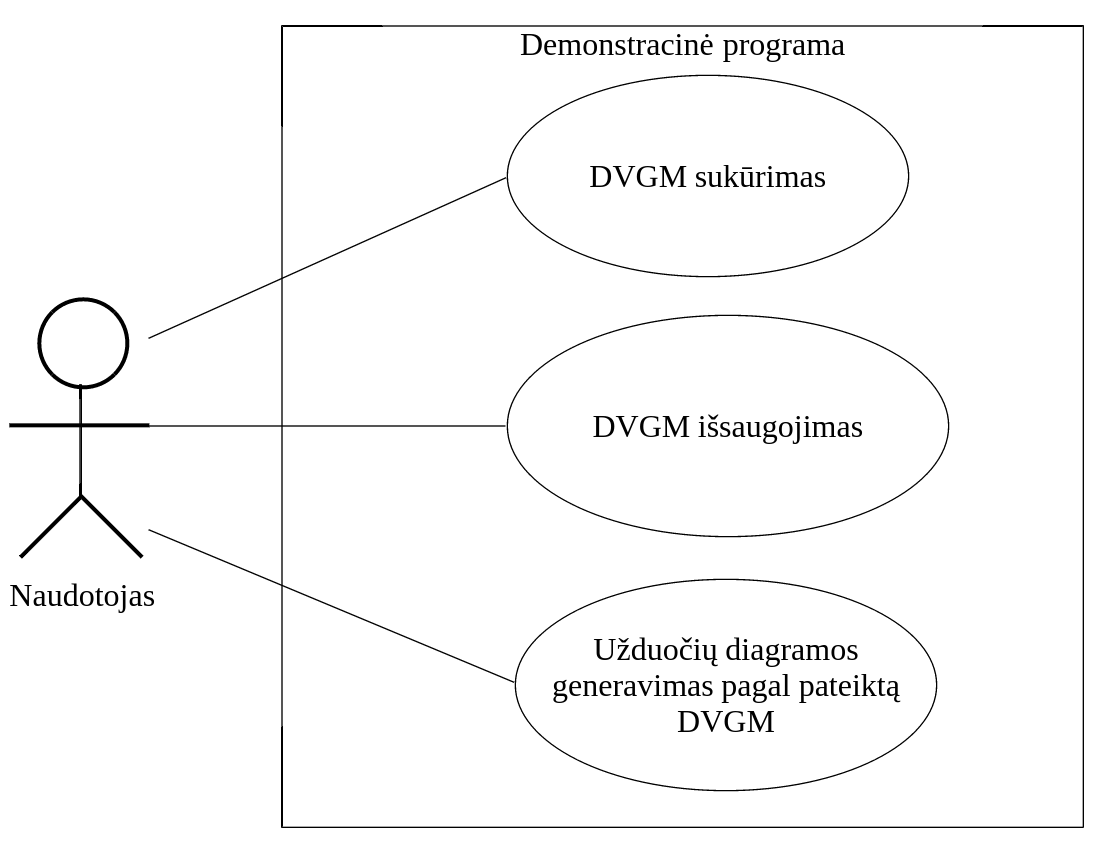
\includegraphics[width=\textwidth]{sections/prototype_app/img/program_functional_requirements}
	\caption{Demonstracinės programos funkciniai reikalavimai.}
	\label{img:program_functional_requirements}
\end{figure}

\begin{center}
    \begin{longtable}{|p{\textwidth}|}
    \caption{\DVCM{} kūrimo naudojimo atvejis}
	\label{tab:program_re_dvcm_creation}
	\\ \hline
    \begin{tabular}{@{}p{3.5cm}p{12cm}}
    	\\
    	\textbf{ID} & NA1
    	\\
    	\textbf{Pavadinimas} & \DVCM{} sukūrimas
    	\\
    \end{tabular}
    \\
    \textbf{Aktoriai}
    \begin{enumerate}
    	\item Naudotojas.
	\end{enumerate}
    \\
    \textbf{Aprašas}

      Naudotojas pasinaudojęs demonstracine programa sukuria \DVCM{}.

    \\
    \textbf{Prieš sąlygos}
    \begin{enumerate}
    	\item Naudotojas yra atidaręs demonstracinės programos langą.
	\end{enumerate}
    \\
    \textbf{Priežastys}
    \begin{enumerate}
    	\item Naudotojas pareikalavo sukurti \DVCM{}.
	\end{enumerate}
    \\
    \textbf{Po sąlygos}
    \begin{enumerate}
    	\item Naudotojas yra sukūręs \DVCM{}.
      \item Naudotojas mato savo sukurtą \DVCM{} demonstracinės programos lange.
	\end{enumerate}
    \\
    \textbf{Pagrindinė užduočių seka}
    \begin{enumerate}
    	\item Demonstracinė programa pateikia interfeisą \DVCM{} kūrimui.
    	\item Naudotojas kuria \DVCM{}.
	\end{enumerate}
    \\
    \textbf{Alternatyvios užduočių sekos}

    \\
    \textbf{Išimtinės užduočių sekos}

    \\
    \\ \hline
    \end{longtable}
\end{center}

\begin{center}
    \begin{longtable}{|p{\textwidth}|}
    \caption{\DVCM{} saugojimo naudojimo atvejis}
	\label{tab:program_re_dvcm_save}
	\\ \hline
    \begin{tabular}{@{}p{3.5cm}p{12cm}}
    	\\
    	\textbf{ID} & NA2
    	\\
    	\textbf{Pavadinimas} & \DVCM{} išsaugojimas
    	\\
    \end{tabular}
    \\
    \textbf{Aktoriai}
    \begin{enumerate}
    	\item Naudotojas.
	\end{enumerate}
    \\
    \textbf{Aprašas}

      Naudotojas išsaugo demonstracine programa sukurtą \DVCM{}.

    \\
    \textbf{Prieš sąlygos}
    \begin{enumerate}
    	\item Naudotojas yra atidaręs \DVCM{} kūrimo interfeisą.
	\end{enumerate}
    \\
    \textbf{Priežastys}
    \begin{enumerate}
    	\item Naudotojas pareikalavo išsaugoti \DVCM{}.
	\end{enumerate}
    \\
    \textbf{Po sąlygos}
    \begin{enumerate}
    	\item Naudotojas yra išsaugojęs \DVCM{}.
      \item Naudotojas žino, kad \DVCM{} išsaugotas.
	\end{enumerate}
    \\
    \textbf{Pagrindinė užduočių seka}
    \begin{enumerate}
    	\item Demonstracinė programa pateikia išsaugojimo formatus.
    	\item Naudotojas pasirenka kaip saugoti \DVCM{}.
			\item Demonstracinė programa pareikalauja išsaugojimo informacijos.
			\item Naudotojas įveda išsaugojimo informaciją.
      \item Demonstracinė programa išsaugo \DVCM{}.
      \item Demonstracinė programa patvirtina, kad \DVCM{} išsaugotas.
	\end{enumerate}
    \\
    \textbf{Alternatyvios užduočių sekos}

    \\
    \textbf{Išimtinės užduočių sekos}
			\newlist{seka}{enumerate}{3}
			\setlist[seka]{label*=\arabic*.,leftmargin=2em}
			\setlist[seka,1]{label=*.\arabic*.,leftmargin=2em}
			\begin{seka}
					\item Naudotojas atsisako išsaugoti \DVCM{}.
					\begin{seka}
						\item Naudotojas pateikia išsaugoti atsisakymą.
						\item Demonstracinė programa nebereikalauja duomenų.
					\end{seka}
			\end{seka}
    \\
    \\ \hline
    \end{longtable}
\end{center}

\begin{center}
    \begin{longtable}{|p{\textwidth}|}
    \caption{Užduočių diagramos generavimo pagal pateiktą \DVCM{} modelį naudojimo atvejis}
	\label{tab:program_re_uc_generation}
	\\ \hline
    \begin{tabular}{@{}p{3.5cm}p{12cm}}
    	\\
    	\textbf{ID} & NA3
    	\\
    	\textbf{Pavadinimas} & Užduočių diagramos generavimas pagal pateiktą \DVCM{}
    	\\
    \end{tabular}
    \\
    \textbf{Aktoriai}
    \begin{enumerate}
    	\item Naudotojas.
	\end{enumerate}
    \\
    \textbf{Aprašas}

      Naudotojas demonstracinei programai programa pateikia \DVCM{} ir programa sugeneruoja užduočių diagramą.

    \\
    \textbf{Prieš sąlygos}
    \begin{enumerate}
    	\item Naudotojas yra atidaręs programos langą.
	\end{enumerate}
    \\
    \textbf{Priežastys}
    \begin{enumerate}
    	\item Naudotojas pareikalavo sugeneruoti užduočių diagramą iš \DVCM{}.
	\end{enumerate}
    \\
    \textbf{Po sąlygos}
    \begin{enumerate}
    	\item Demonstracinėje programoje yra užduočių diagramos duomenys.
      \item Naudotojas mato sugeneruotą užduočių diagramą Demonstracinės programos lange.
	\end{enumerate}
    \\
    \textbf{Pagrindinė užduočių seka}
    \begin{enumerate}
      \item Demonstracinė programa pateikia užduočių diagramos generavimo iš \DVCM{} variantus.
      \item Naudotojas pasirenka generuoti bendrą diagramą iš \DVCM{}. \label{seka:re_generate_choose_way}
    	\item Demonstracinė programa pateikia interfeisą \DVCM{} įvedimui.
    	\item Naudotojas įveda \DVCM{}.
      \item Demonstracinė programa sugeneruoja užduočių diagramos modelį.
      \item Demonstracinė programa pavaizduoja užduočių diagramą lange.
	\end{enumerate}
    \\
    \textbf{Alternatyvios užduočių sekos}
			\newlist{seka}{enumerate}{3}
			\setlist[seka]{label*=\arabic*.,leftmargin=2em}
			\setlist[seka,1]{label=\ref{seka:re_generate_choose_way}.\arabic*.,leftmargin=2em}
			\begin{seka}
					\item Naudotojas Naudotojas pasirenka iš \DVCM{} sugeneruotą diagramą rodyti po vieną transakciją.
			\end{seka}
    \\
    \textbf{Išimtinės užduočių sekos}
			\newlist{seka}{enumerate}{3}
			\setlist[seka]{label*=\arabic*.,leftmargin=2em}
			\setlist[seka,1]{label=*.\arabic*.,leftmargin=2em}
			\begin{seka}
					\item Naudotojas atsisako generavimo.
					\begin{seka}
						\item Naudotojas pateikia generavimo atsisakymą.
						\item Demonstracinė programa nebereikalauja duomenų.
					\end{seka}
			\end{seka}
    \\
    \\ \hline
    \end{longtable}
\end{center}

\subsection{Technologijos pasirinktos programos įgyvendinimui}

\subsubsection{Javascript}

Programai įgyvendinti pasirinkta „Javascript“ programavimo kalba. Kadangi reikės atvaizduoti diagramas buvo nuspręsta atlikti tai panaudojant HTML galimybes.  „Javascript“ yra aukšto lygio programavimo kalba. Naujausios jos versijos yra objektiškai orientuotos ir pateikia nemažai kitų aukšto lygio abstrakcijų. Ši kalba yra silpnai tipizuota, objektų išplėtimams naudoja prototipus. „Javascript“ suteikia naršyklių rodomiems puslapiams dinamiškumą. Ilgą laiką ji buvo naudojama tik tam, bet kalbai išpopuliarėjus, ją imta taikyti ir srityse kaip serverinės ar net darbastalio programos. „Javascript“ naudojama kaip interpretuojama programavimo kalba. Interpretavimo standartas „ECMAScript“ buvo išleistas 1997 metais, nuo to laiko jis smarkiai pasikeitė. 2018 metais labiausiai naršyklių pilnai palaikomas yra 5 standartas, šiame darbe rašomas kodas bus transliuojamas į jį.
%Programa yra pilnai klientinės puses (client side), ji neturi serverinės dalies (backend), yra galimybė generuoti failus sukurtiems duomenims saugoti. Failai yra JSON arba JPG formato.

Programos „Javascript“ kodui rašyti pasirinkta 6 „ECMAScript“ versija \cite{EcmaScript}.

\subsubsection{Node.js}

Pasirinkta atviro kodo „Node.js“ programavimo aplinka \cite{nodeJs}. Ši aplinka pritaikyta dirbti su „Javascript“ projektais. Išoriniams paketams tvarkyti pasirinkta atviro kodo „NPM“ paketų tvarkyklė \cite{npmWebsite}. Ši tvarkyklė padeda tvarkyti „Javascript“ paketų versijas. Ji buvo pasirinkta nes yra pagrindinė „Node.js“ aplinkos paketų tvarkyklė.


\subsubsection{Webpack}

Programos modelių surinkimas ir transliavimas aprašomas naudojant atviro kodo „Javascript“ modulių surinkimo bibliotekos „Webpack“ konfiguraciją \cite{webpack}. Ji leidžia pasirinkti kokie moduliai ir kokiu būdu turi būti surinkti ir transliuoti. „Webpack“ naudojamas surinkti „Javascript“ projektą iš daugybės modulių ir transliuoti juos taip, kad palaikytų norimą versiją. Šiuo atveju „Javascript“ 6 standarto kodas transliavimas į 5, kad veiktų naršyklėse.

\subsubsection{Babel}

Programos kodas transliuojamas atviro kodo transliatoriumi „Babel“, kuris naudojamas kaip „Webpack“ prijungimas (plugin).


\subsubsection{MobX}

Programa modeliuojama naudojant MVC metodologiją. Modeliui ir kontroleriui pasirinkta atviro kodo „MobX“ modeliavimo biblioteka \cite{githubMobX}. Ji leidžia kurti programos duomenų modelius ir kontroliuoja jų būsenos klausymąsi naudodama „Javascript“ objekto duomenų priskyrimo ir gavimo metodus.

\subsubsection{React}

Programos „MVC“ vaizdavimo dalis kuriama naudojant atviro kodo „React“ biblioteką \cite{reactJs}. Ji pateikia patogų virtualaus dokumento objekto modelio interfeisą kuris pritaikytas veikti vienodai visose naršyklėse ir optimizuoja dokumento objekto modelio atnaujinimus. Taip pat turi patogią sintaksę vaizdo apibrėžimui – „JSX“. „React“ labai gerai integruojasi su „MobX“.

\subsection{Programos veikimo pavyzdžiai}

\lstset{language=Java,keywordstyle={\bfseries \color{blue} \textbf}}

Atidarius programą matomas trumpas jos aprašymas. Programą galima lokalizuoti į konsolę įvedus komandą \inCode{editorModel.locale = "lt_LT"} (priedas \ref{appendix:run_examples_welcome}). Programa pateikia grafinę diagramų atvaizdavimo sąsają, bet jų kūrimui pateikiamas komandinis interfeisas. Komandomis vadinami „window“ objektui priskirti programos objektai (naudojimo pavyzdys: kodas \ref{lst:commands_to_create_dvcm}). Paspaudus mygtuką \uiWord{Naujas} matomas diagramos kūrimo langas (priedas \ref{appendix:run_examples_new}). Pasirinkus \uiWord{\DVCM{}} rodomas \DVCM{} kūrimo sąsaja (priedas \ref{appendix:run_examples_new_dvcm}). Joje galimos \DVCM{} redagavimo komandos. Suvedus komandas iš \ref{lst:commands_to_create_dvcm} kodo gaunamas \DVCM{} modelis. Šiek tiek pakoreguotas grafine sąsaja jis pavaizduotas priede \ref{appendix:run_examples_created_dvcm}. Sudėtingesnio \DVCM{} (priedas \ref{appendix:dvcm_window}) \JSON{} formato duomenų failas yra pateiktas \href{https://aleksandras-sivkovas.github.io/diagrams-editor-app/dvcm.json}{https://aleksandras-sivkovas.github.io/diagrams-editor-app/dvcm.json}.

\renewcommand{\lstlistingname}{Kodas}
\renewcommand{\lstlistlistingname}{Kodo fragmentai}
\setcounter{lstlisting}{0}
\lstinputlisting[style=javascript, caption={Komandos gauti \ref{appendix:run_examples_created_dvcm} priede pavaizduotą \DVCM}, label={lst:commands_to_create_dvcm}]{sections/prototype_app/code/commands_for_dvcm.js}




\sectionnonum{Rezultatai ir išvados}

\begin{enumerate}
  \item Iš literatūros analizės apie reikalavimų inžineriją nustatytas reikalavimų inžinerijos aktualumas. Taip pat nustatytas įrankių reikalavimų inžinerijai aktualumas. Įrankis leistų:
  \begin{enumerate}
    \item Sumažinti žmogiškąjį klaidos faktorių. Automatizavus procesą žmogus gautų teoriškai teisingus reikalavimus.
    \item Paspartinti reikalavimų inžinerijos procesą.
    \item Padaryti reikalavimus prieinamus visiem komandos nariam. Visi žinotų koks yra projekto statusas.
    \item Sekti reikalavimų pasikeitimus.
  \end{enumerate}
  \item Pagal modeliavimo kalbų standartų ir transformavimo algoritmų analizę nustatyta, kad trūksta \BPMN{} transformavimo į užduočių diagramą algoritmo. Rastas algoritmas, kuris atlieka transformaciją remdamasis empirinėmis taisyklėmis.
  \item Kadangi daugelis \BPMN{} komponentų neturi įtakos užduočių diagramos generavimo rezultatui išanalizavus \BPMN{} standartą sudarytas \BPMN{} pagrindinių komponentų metamodelis. Jis apibūdina algoritmo įvesties duomenis.
  \item Išanalizavus \UML{} ir \SysML{} standartus sudarytas užduočių diagramos metamodelis. Jis apibūdina algoritmo rezultatą.
  \item Pasiūlytas \BPMN{} standarto praplėtimas. Parodyta kokios anksčiau aprašyto algoritmo problemos išsisprendžia generuojant užduočių diagramą pagal \BPMN{} sukurtą pagal \DVCM{} teoriją.
  \item Išanalizavus modeliavimo kalbų standartus ir egzistuojančius algoritmus pasiūlytas \BPMN{} transformavimo į užduočių diagramą algoritmas, kuris sukonstruoja užduočių diagramos modelį. Pateikiamas algoritmo pseudokodas bei jį apibūdinanti veiklos diagrama. Sukurtas algoritmas galėtų būti pritaikytas reikalavimų inžinerijos įrankyje.
  \item Sukurta demonstracinė programa leidžianti:
  \begin{enumerate}
    \item Kurti \BPMN{} pagal \DVCM{} teoriją.
    \item Iš sukurto modelio generuoti užduočių diagramą.
  \end{enumerate}
\end{enumerate}

%Šiame skyriuje pateikiamos išvados (reziume) anglų kalba.
%\sectionnonum{Conclusions}
\printbibliography[heading=bibintoc] % Literatūros šaltiniai aprašomi

\sectionnonum{Santrumpos}
Šiame darbe naudojami žymėjimai:
\begin{enumerate}
	%\item \BPMN{} – modeliavimo kalba, skirta pavaizduoti informaciją plačiai auditorijai. \BPMN{} buvo sukurta ir dažniausia naudojama pavaizduoti verslo procesams \cite{bpmnFormal}.
	\item \textbf{UML} – modeliavimo kalba, skirta suteikti standartinį sistemos analizės, architektūros, veikimo ir kūrimo pavaizdavimą \cite{omgUmlFormal}. \label{def:uml}
	\item \textbf{SysML} – \UML{} išplėtimas skirtas modeliuoti programų sistemas. \cite{OMGSysML} \label{def:sysml}
	%\item \textbf{Sekų diagrama} (angl. sequence diagram) – \UML{} diagrama, skirta pavaizduoti žinučių tarp apibrėžtų objektų sekai tų objektų gyvavimo metu \cite{omgUmlFormal}.
	%\item Užduočių diagrama (angl. use case diagram) – \UML{} diagrama, skirta pavaizduoti pavaizduoti kaip gali būti naudojama programų sistema \cite{algUseCasesFromBpmn}.
	\item \textbf{OMG} (angl. Object Management Group) – atviras, tarptautinis ne pelno siekiantis technologijų standartų konsorciumas (https://www.omg.org/). \label{def:omg}
	%\item \textbf{DVGM} – Detalizuotas grandinės vertės modelis, transakcinių darbų sekų modelis, \BPMN{} modelio praplėtimas atskiriantis įmonės procesus ir valdymo funkcijas kaip M. Porterio modelis ir suskirstantis juos į valdymo transakcijas.
  \item \textbf{JSON} (angl. JavaScript Object Notation) – atviras failo formato standartas naudojantis žmogui perskaitomą tekstą duomenims koduoti. \label{def:json}
\end{enumerate}

\appendix  % Priedai

\section{Vertės grandinės modelis programos lange} \label{appendix:dvcm_window}
\JSON{} formato duomenų failas yra pateiktas \href{https://aleksandras-sivkovas.github.io/diagrams-editor-app/dvcm.json}{https://aleksandras-sivkovas.github.io/diagrams-editor-app/dvcm.json}.
\begin{figure}[H]
    \centering
    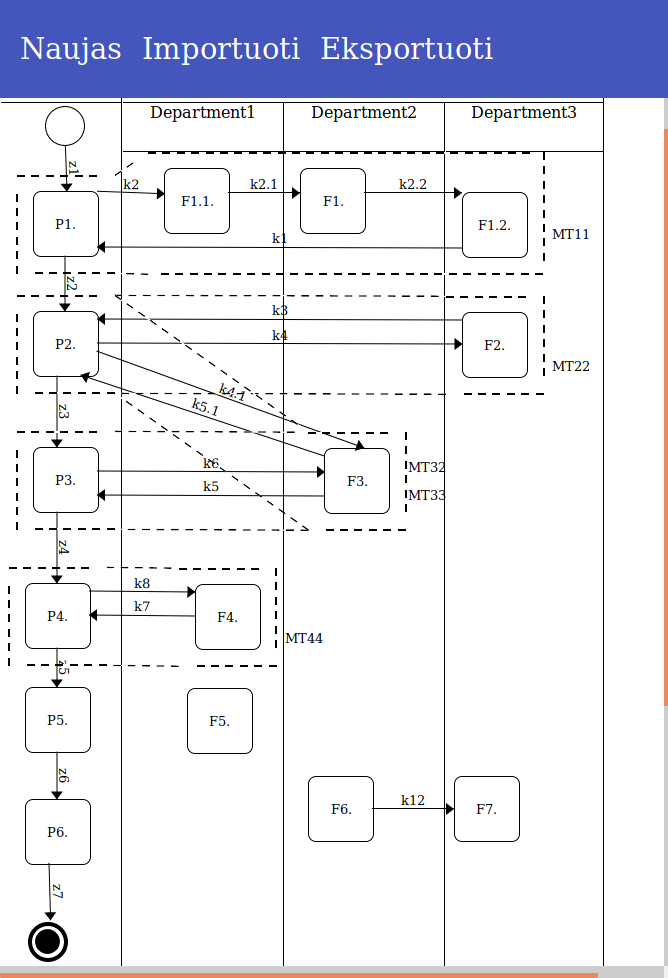
\includegraphics[height=20cm]{img/dvcm_window}
\end{figure}

\section{\ref{appendix:dvcm_window} priedo užduočių diagramos} \label{appendix:use_cases_window}
Iš \ref{appendix:dvcm_window} priedo \DVCM{} transformuotos užduočių diagramos.

\begin{figure}[H]
    \centering
    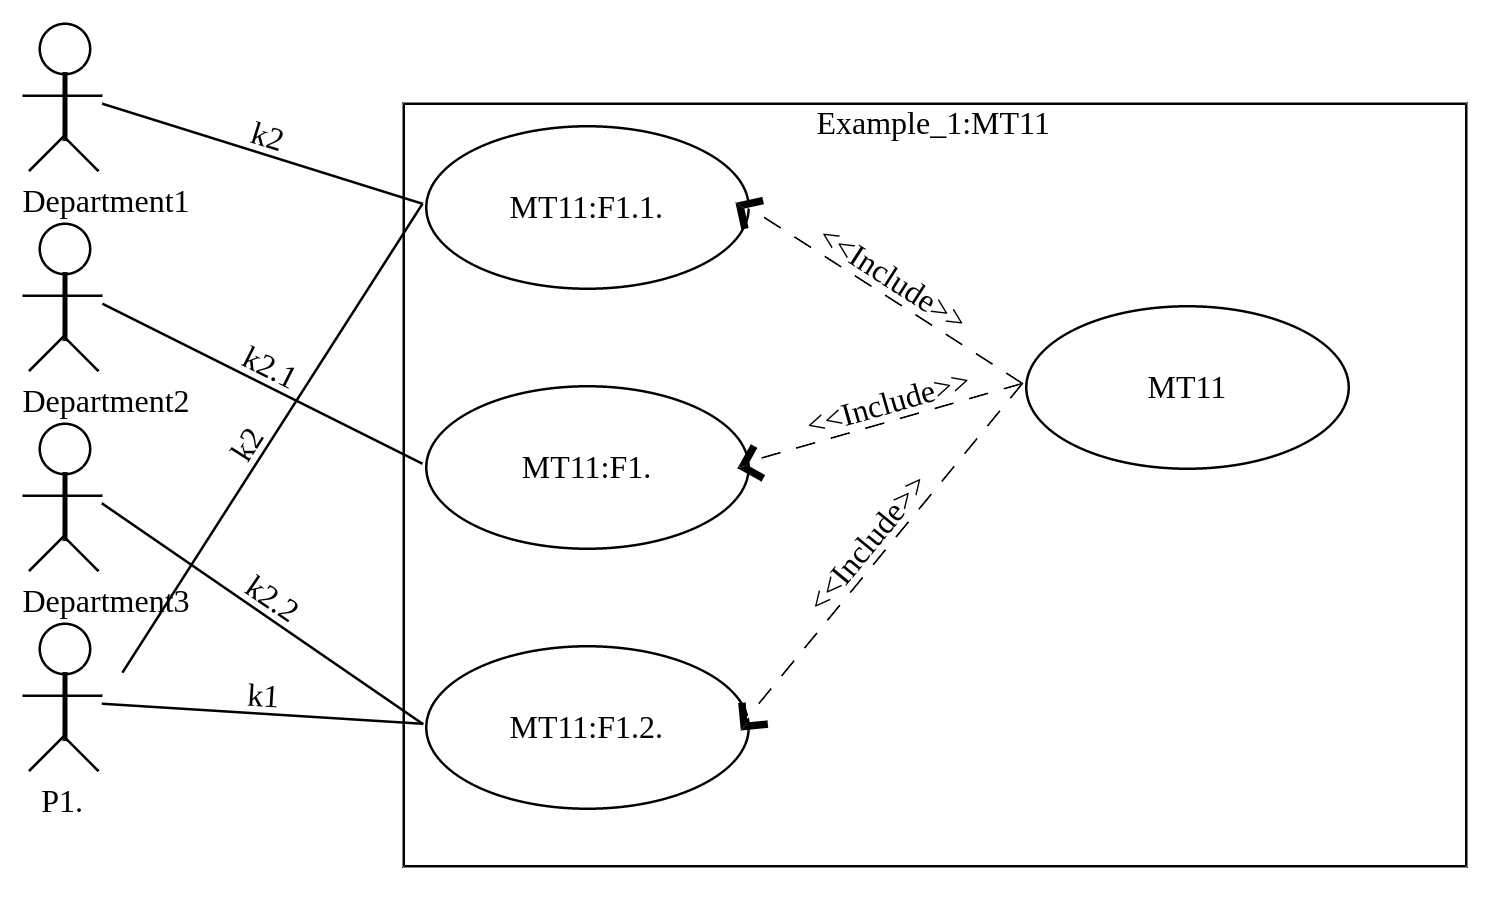
\includegraphics[width=12cm]{img/appendix/run_examples/generated_use_case/mt11}
\end{figure}
\begin{figure}[H]
    \centering
    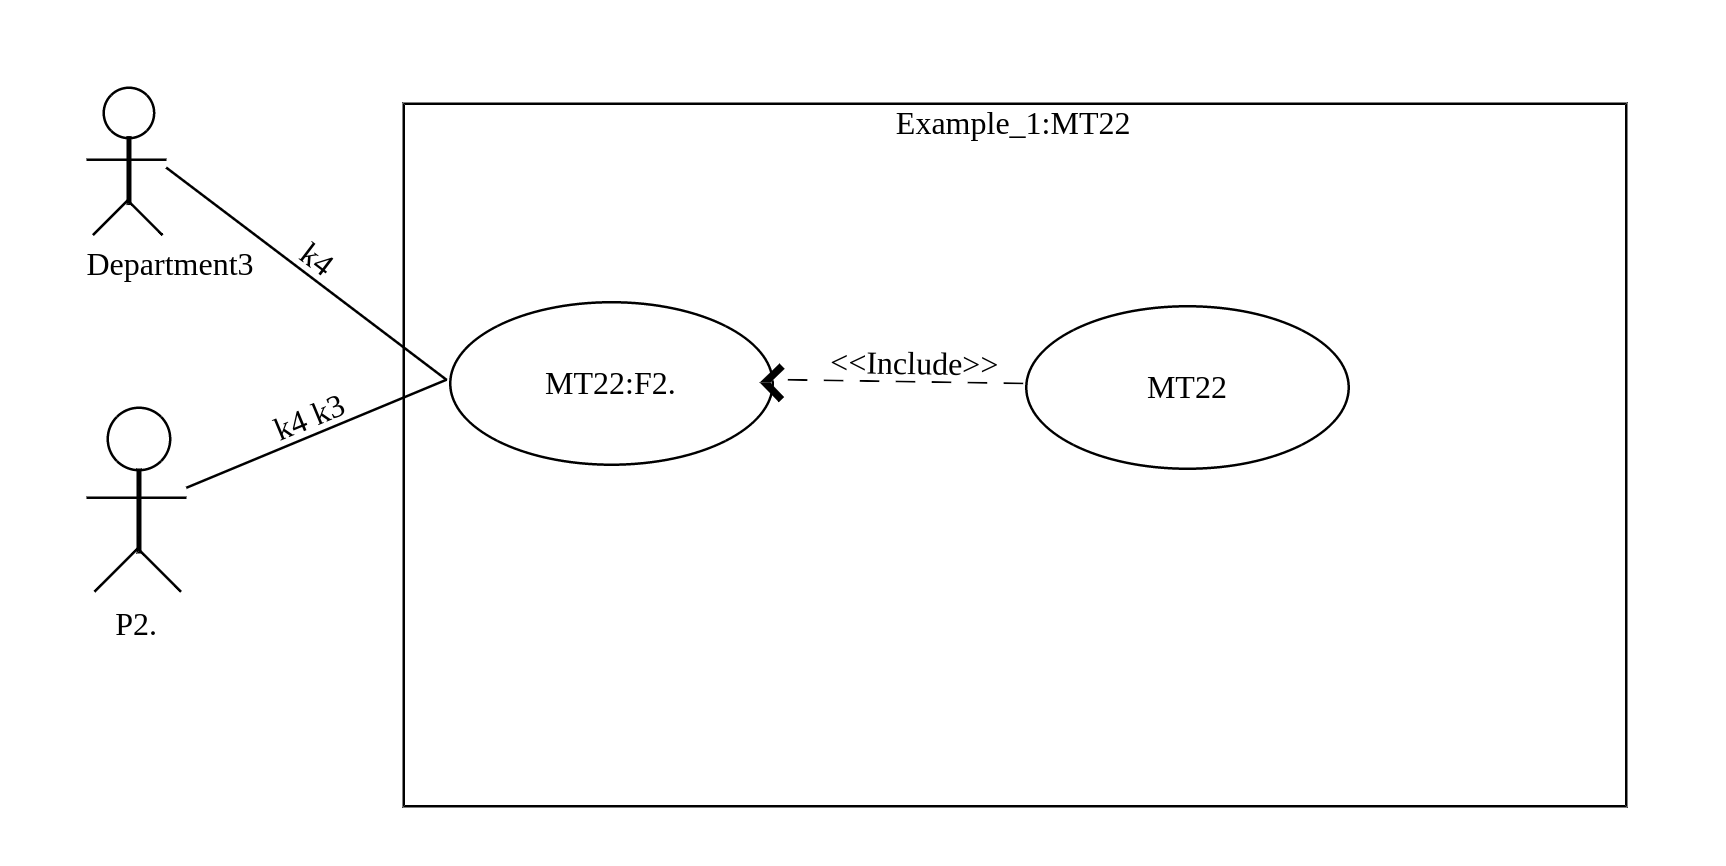
\includegraphics[width=12cm]{img/appendix/run_examples/generated_use_case/mt22}
\end{figure}
\begin{figure}[H]
    \centering
    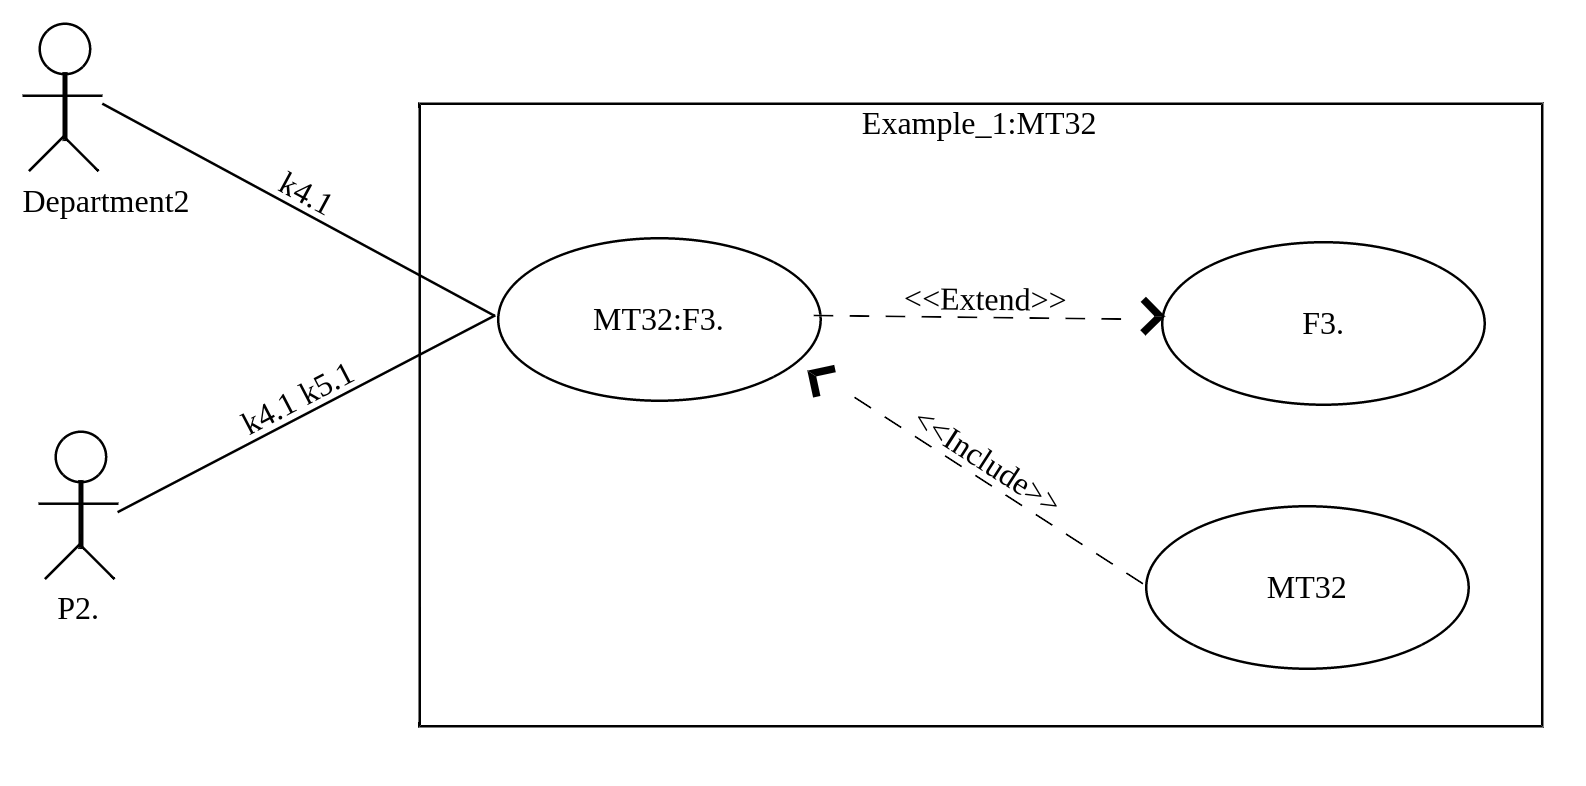
\includegraphics[width=12cm]{img/appendix/run_examples/generated_use_case/mt32}
\end{figure}
\begin{figure}[H]
    \centering
    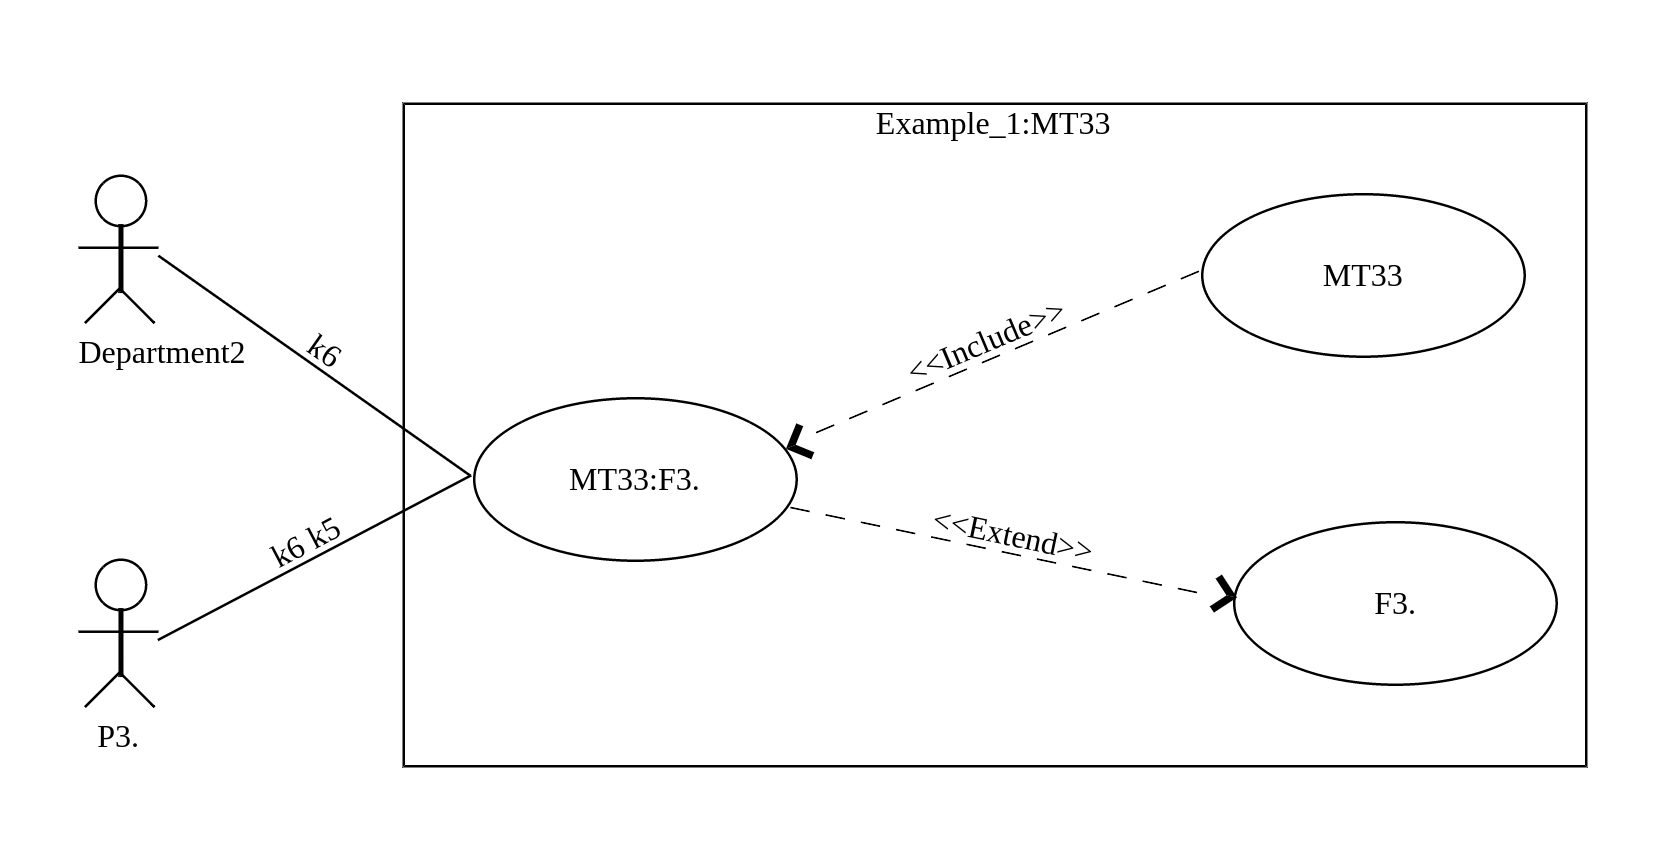
\includegraphics[width=12cm]{img/appendix/run_examples/generated_use_case/mt33}
\end{figure}
\begin{figure}[H]
    \centering
    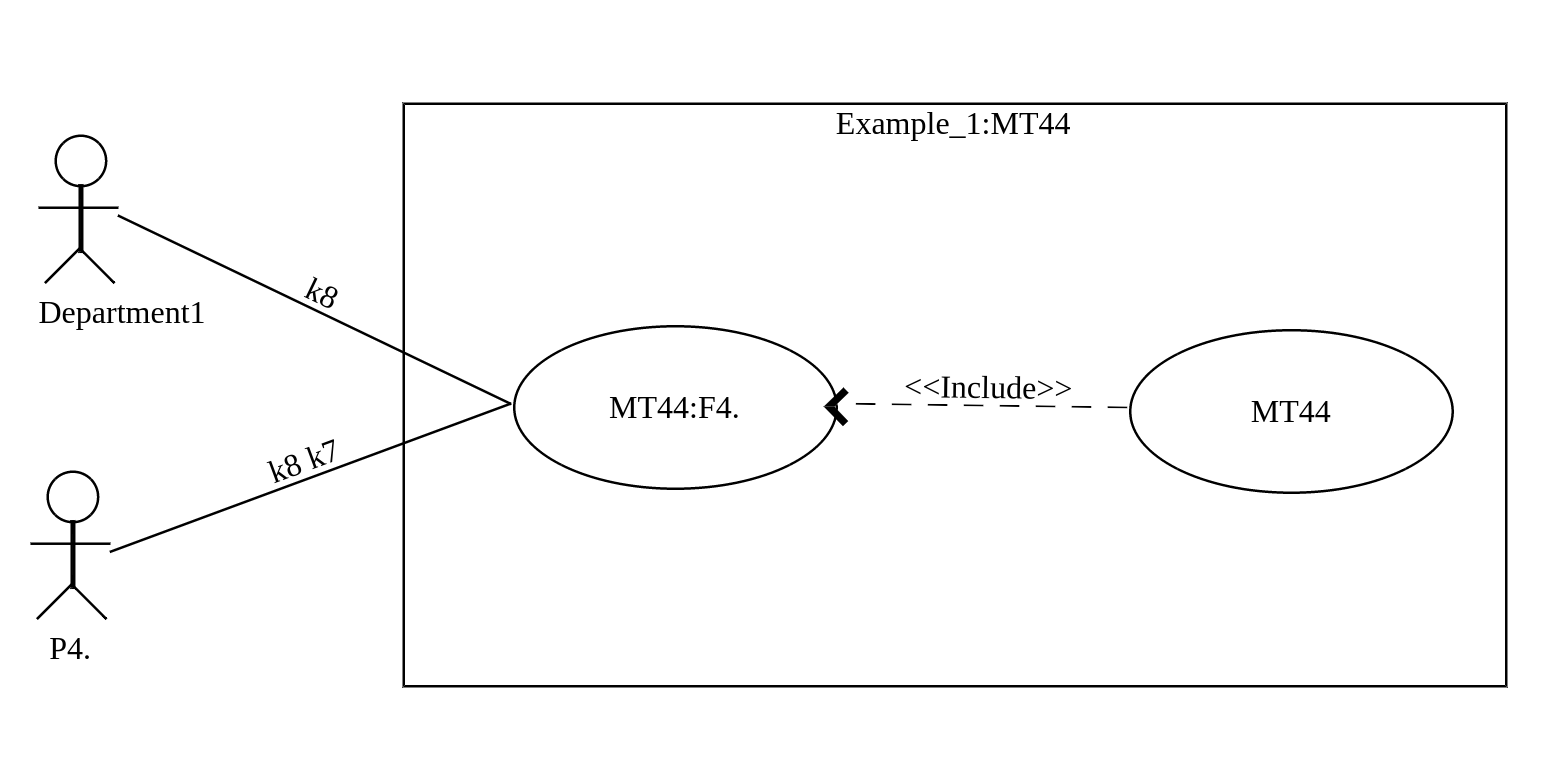
\includegraphics[width=12cm]{img/appendix/run_examples/generated_use_case/mt44}
\end{figure}
\begin{figure}[H]
    \centering
    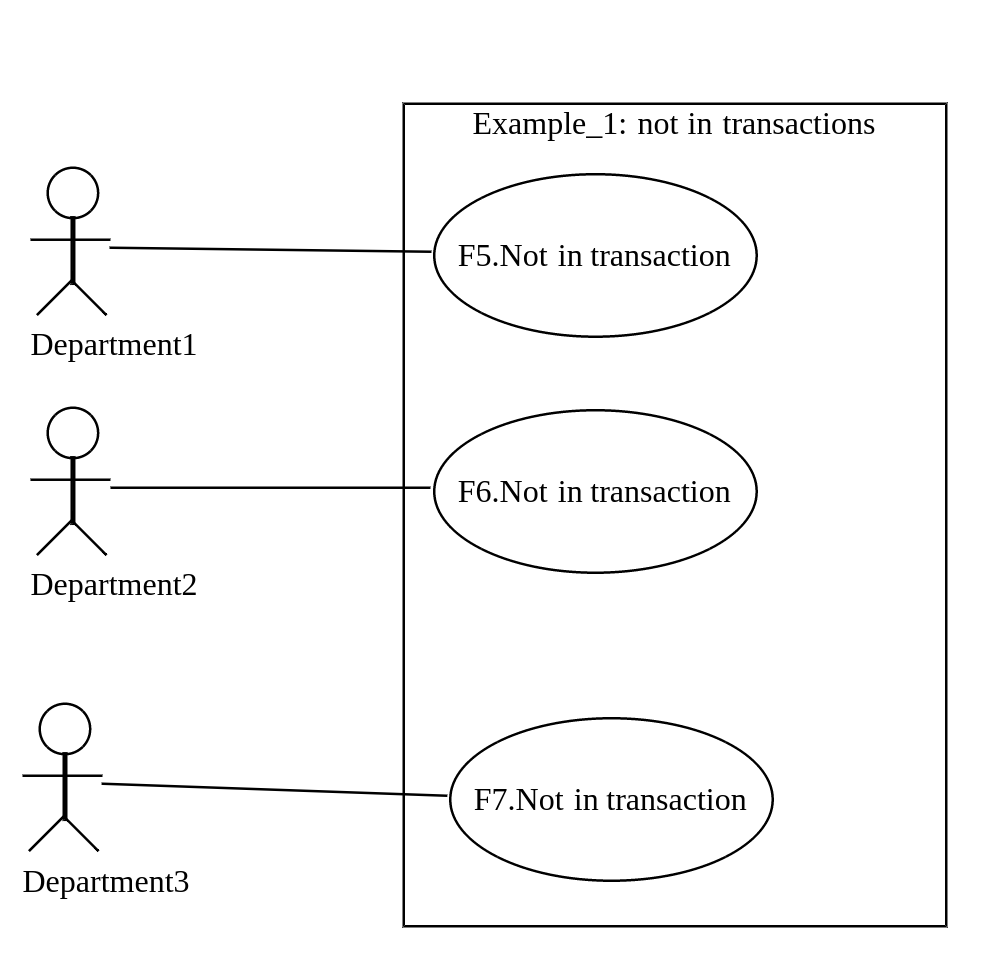
\includegraphics[width=10cm]{img/appendix/run_examples/generated_use_case/not_in_transaction}
\end{figure}

\section{Užduočių diagramos metamodelis} \label{appendix:lit_alg_metamodels_uc}

Čia pateikiamas literatūroje rasto algoritmo straipsnio \cite{algUseCasesFromBpmn} pateiktas Užduočių diagramos (Use case) metamodelis.

\begin{figure}[H]
    \centering
    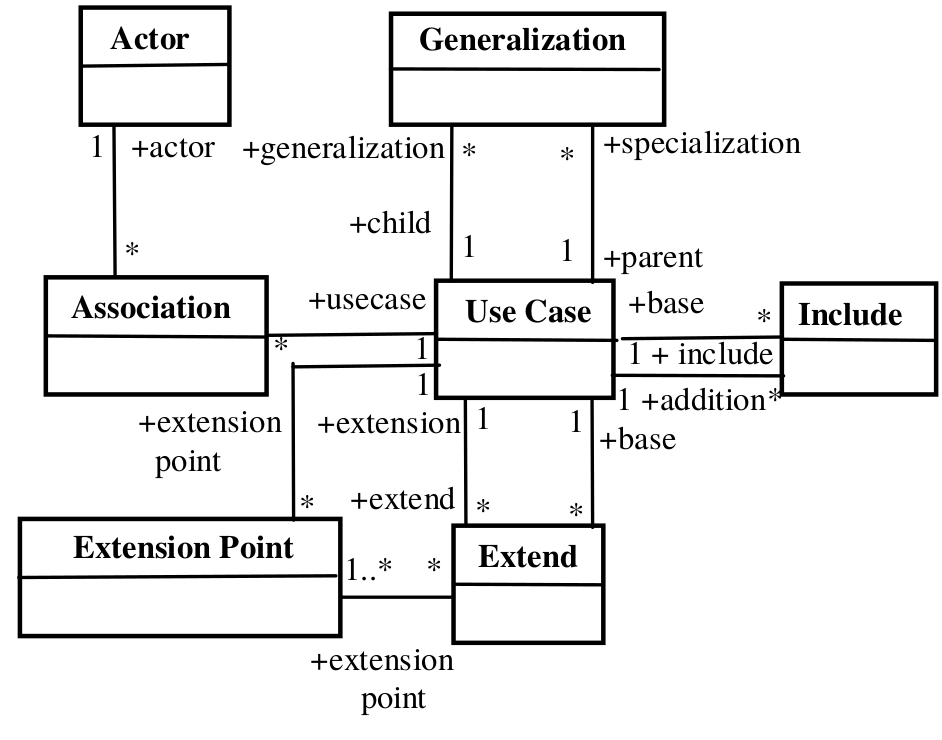
\includegraphics[width=\textwidth]{img/appendix/literature_algorythm/use_cases_metamodel}
    \caption{Užduočių diagramos metamodelis}
\end{figure}

\section{BPMN metamodelis} \label{appendix:lit_alg_metamodels_bpmn}

Čia pateikiamas literatūroje rasto algoritmo straipsnio \cite{algUseCasesFromBpmn} pateiktas \BPMN{} metamodelis.

\begin{figure}[H]
    \centering
    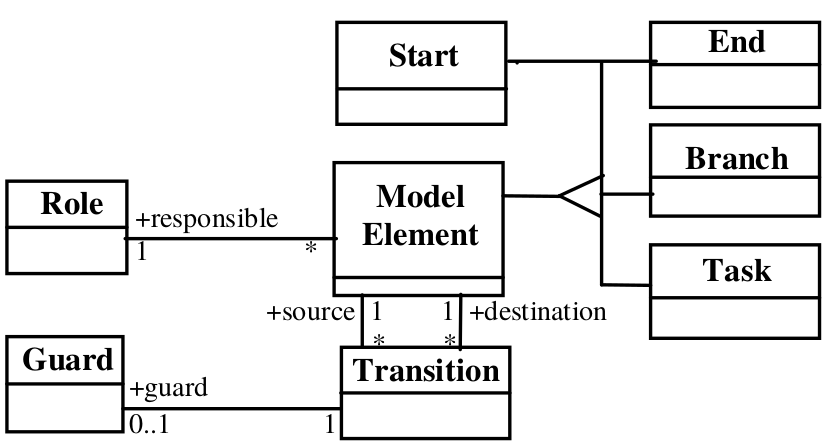
\includegraphics[width=\textwidth]{img/appendix/literature_algorythm/bpmn_metamodel}
\end{figure}

\section{Inttegruotas metamodelis} \label{appendix:lit_alg_metamodels_integrated}
Čia pateikiamas literatūroje rasto algoritmo straipsnio \cite{algUseCasesFromBpmn} pateiktas integruotas \BPMN{} ir užduočių diagramos (Use case) metamodelis.
\begin{figure}[H]
    \centering
    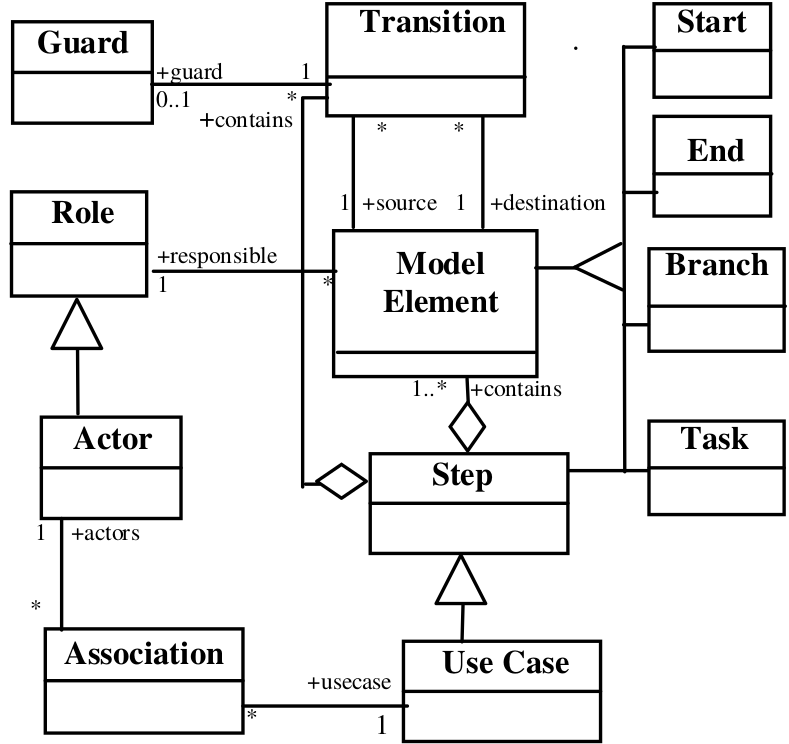
\includegraphics[width=\textwidth]{img/appendix/literature_algorythm/integrated_metamodel}
\end{figure}

\section{Langas matomas atidarius programą} \label{appendix:run_examples_welcome}
\begin{figure}[H]
    \centering
    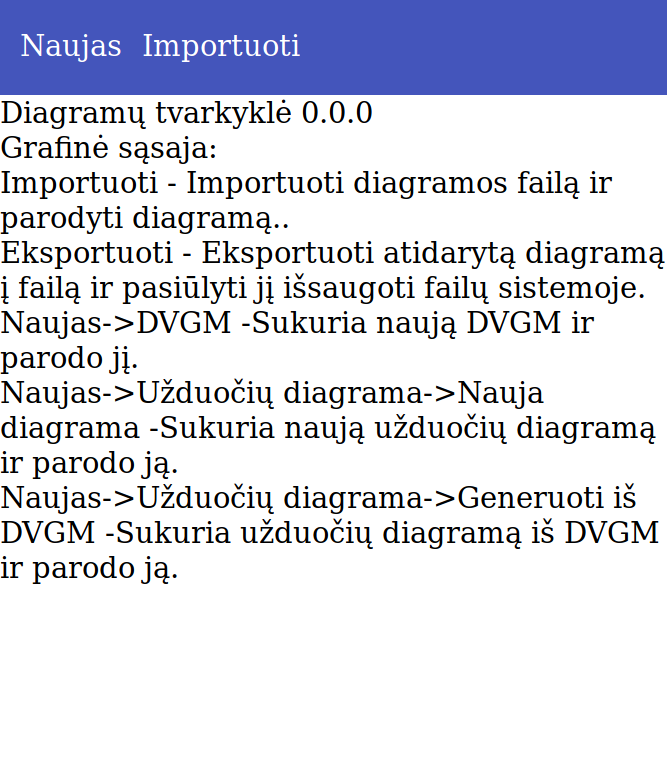
\includegraphics[height=20cm]{img/appendix/run_examples/welcome}
\end{figure}

\section{Sukūrimo sąsaja} \label{appendix:run_examples_new}
\begin{figure}[H]
    \centering
    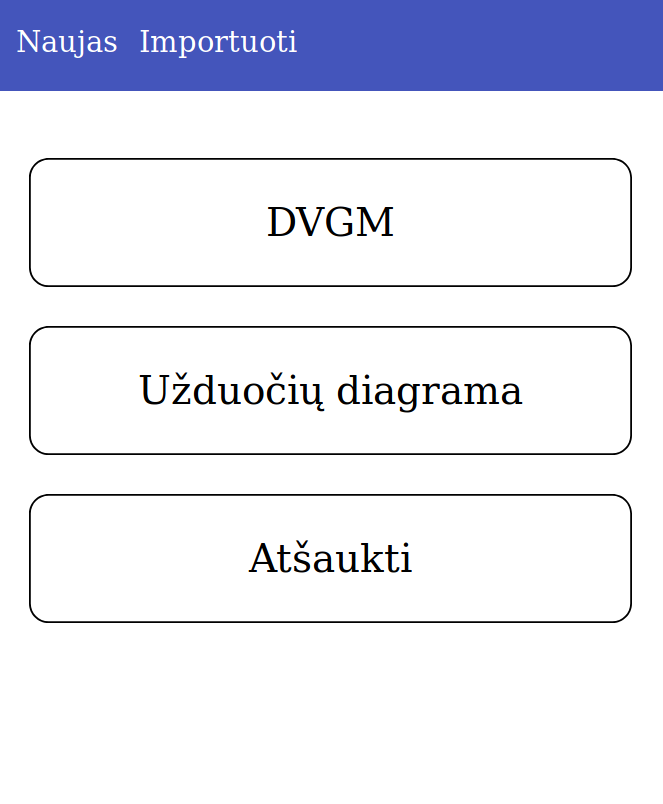
\includegraphics[height=20cm]{img/appendix/run_examples/new}
\end{figure}

\section{DVGM Kūrimo sąsaja} \label{appendix:run_examples_new_dvcm}
\begin{figure}[H]
    \centering
    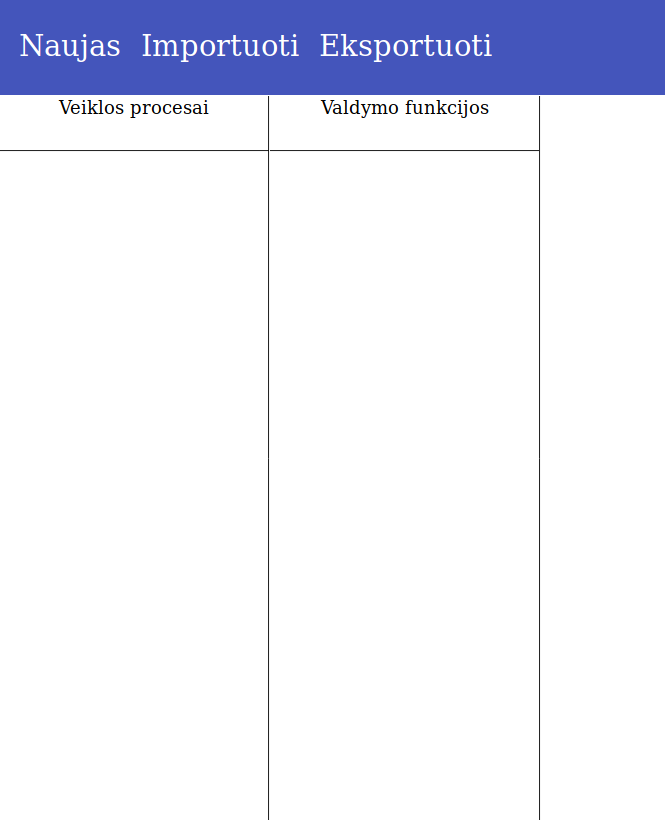
\includegraphics[height=20cm]{img/appendix/run_examples/new_dvcm}
\end{figure}

\section{Sukurto DVGM pavyzdys} \label{appendix:run_examples_created_dvcm}
\begin{figure}[H]
    \centering
    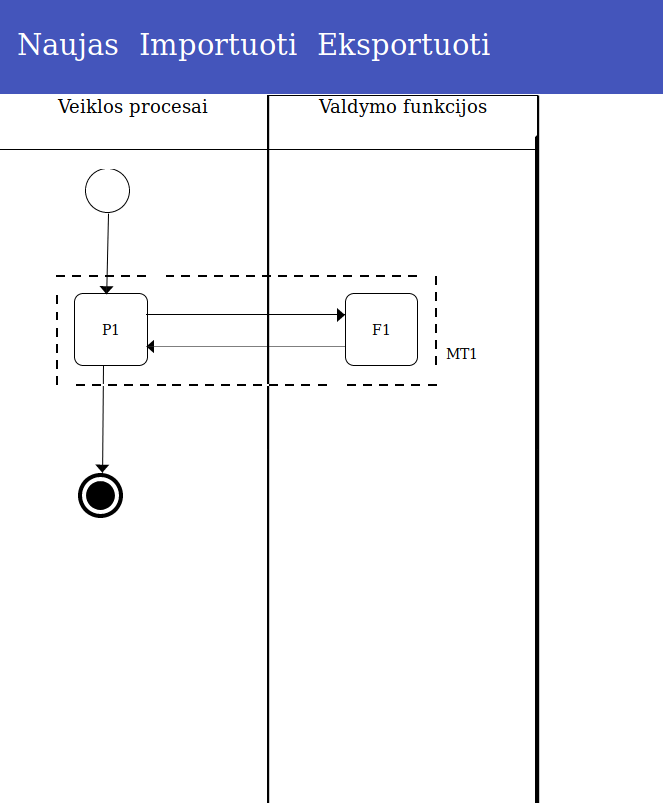
\includegraphics[height=20cm]{img/appendix/run_examples/created_dvcm}
\end{figure}


\section{Pseudokodo realizacija Javascript kalba} \label{appendix:pseudocode_implementation}
Algoritmo aprašyto \ref{section:main_use_cases_from_bpmn} skyriuje realizaciją „Javascript“ kalba.
\lstinputlisting[style=javascript]{UseCasesFromDvcmDataGenerator.js}

\end{document}
